\documentclass[12pt,a4paper,openright,twoside]{book}
\usepackage[utf8]{inputenc}
\usepackage{amsmath}
\usepackage{amssymb}
\usepackage{listings}
\usepackage{algorithm}
\usepackage{algpseudocode}
\usepackage{tabularx}
\usepackage{graphics}
\usepackage{disi-thesis}
\usepackage{code-lstlistings}
\usepackage{notes}
\usepackage{shortcuts}
\usepackage{acronym}
%\usepackage[linesnumbered,ruled,vlined]{algorithm2e}


\newcommand{\thesislang}{english} % commentare in caso di tesi in italiano
%\usepackage{thesis-style}
% version
%\newcommand{\versionmajor}{0}
%\newcommand{\versionminor}{1}
%\newcommand{\versionpatch}{2}
%\newcommand{\version}{\versionmajor.\versionminor.\versionpatch}
%\typeout{Document version: \version}

\school{\unibo}
\programme{Corso di Laurea Magistrale in Ingegneria e Scienze Informatiche}
\title{Fair-by-design algoriths for access to education}
\author{Antonio Iannotta}
\date{\today}
\subject{Intelligent Systems Engineering}
\supervisor{Prof. Giovanni Ciatto}
\cosupervisor{Prof. Roberta Calegari}
\morecosupervisor{Prof. Andrea Omicini}
\session{IV}
\academicyear{2022-2023}

% Definition of acronyms
\acrodef{IoT}{Internet of Thing}
\acrodef{vm}[VM]{Virtual Machine}
\acrodef{AI}{Artificial Intelligence}


\mainlinespacing{1.241} % line spacing in mainmatter, comment to default

\begin{document}
	
\frontmatter

% ! TeX root = thesis-main.tex
\title{Title}
\author{Candidate Name Here}
\date{\today}

\newgeometry{margin=0.8in}
\begin{titlepage}
	\begin{center}
		% \vspace*{0.2cm}
		
		\large
		\textbf{ALMA MATER STUDIORUM -- UNIVERSITÀ DI BOLOGNA \\ CAMPUS DI CESENA}
		\\
		\noindent\hrulefill
		\vspace{0.4cm}
		
		\Large
		Scuola di Ingegneria e Architettura \\
		Corso di Laurea Magistrale in Ingegneria e Scienze Informatiche
		
		\Huge
		\vspace{4cm}
		\textbf{
			Fair-by-design algorithm for access to education
		}
		
		\large
		\vspace{1cm}
		Tesi di laurea in 
		\\
		\textsc{Intelligent System Engineering}
		
		\vspace{5.5cm}
		\begin{minipage}[t]{0.64\textwidth}
			\begin{flushleft}
				\textit{Relatore} 
				\\ 
				\textbf{Prof.} \textbf{Giovanni Ciatto}
				\\
				\vspace{0.4cm}
				\textit{Correlatore} 
				\\
				\textbf{Prof.} \textbf{Roberta Calegari}
				\textbf{Prof.} \textbf{Andre Omicini}
			\end{flushleft}
		\end{minipage}
		\begin{minipage}[t]{0.34\textwidth}
			\begin{flushright}
				\textit{Candidato} 
				\\ 
				\textbf{Antonio Iannotta}
			\end{flushright}
		\end{minipage}\\
		
		\vfill
		\noindent\hrulefill
		\vspace{0.3cm}
		\Large
		
		IV Sessione di Laurea
		\\
		Anno Accademico 2022-2023
	\end{center}
\end{titlepage}
\restoregeometry


\begin{abstract}

    This work presents an in-depth approach to address fairness and bias mitigation in the design and development of data-driven methods. The primary contribution of this study is the proposal and implementation of an innovative \emph{Fair-by-Design} workflow that incorporates various strategies for bias mitigation within data, algorithms, and decision-making processes.

    The work focuses on the educational data of the Canary Islands, leveraging a dataset encompassing detailed information about student performance and educational outcomes.

    The primary objective is to ensure equitable and unbiased application of data-driven algorithms within the educational context. 

    The methodology involves the systematic evaluation of multiple bias mitigation strategies. The critical aspect of this research centers on the comparison of these strategies based on their impact on the predictive accuracy of the algorithms. 

    This approach provides practical insights into the trade-offs between fairness and accuracy, showing how several approaches can lead to different accuracy scores on the same dataset and with the same models. 

    The work findings offer valuable insights into the trade-offs between fairness and accuracy when developing data-driven methods for educational data. 

    This thesis contributes to the ongoing discourse on fairness in machine learning and data-driven decision-making. The results provide guidance for stakeholders in the education sector, aiding them in making informed decisions about algorithm deployment to promote fairness and minimize bias within educational systems. 

\end{abstract}
    


%\begin{acknowledgements} % this is optional
%Never too far down, to come back
%\end{acknowledgements}

%----------------------------------------------------------------------------------------
\tableofcontents   
%\listoffigures     % (optional) comment if empty
%\lstlistoflistings % (optional) comment if empty
%----------------------------------------------------------------------------------------

\mainmatter

%----------------------------------------------------------------------------------------
\chapter{Introduction}
\label{chap:introduction}
%----------------------------------------------------------------------------------------

Artificial Intelligence (AI) has experienced an unprecedented surge in prominence and utility in recent years, emerging as a transformative force across diverse domains. From powering autonomous vehicles to aiding healthcare diagnosis and recommendation systems, AI applications have become increasingly woven into the fabric of our daily lives. However, this rapid proliferation has ushered in a pressing concern about the pervasive presence of bias within AI systems.

The concept of bias in AI pertains to the inadvertent or systematic preference shown towards specific groups or characteristics within the data, algorithms, or decision-making processes. This partiality leads to outcomes that are unjust, unfair, and unequal. In this era of AI-driven decision-making, the imperative to address bias is not just a technological challenge but a moral and societal necessity. Additionally, the ethical principle of fairness underscores the collective aspiration to ensure that AI systems yield equitable and just results for all individuals, regardless of their personal attributes.

The repercussions of bias and unfairness in AI systems extend far beyond mere technological concerns. These issues carry profound societal implications, impacting vital areas such as employment, education, and access to critical services. Biased AI systems perpetuate and exacerbate existing inequalities, inadvertently reinforcing harmful stereotypes and undermining the foundational principles of justice and equality.

In the realm of education, data-driven decision-making has gained significant ground, with educational institutions increasingly relying on AI systems for tasks ranging from student admissions to evaluating learning outcomes and allocating educational resources. The stakes in this domain are notably high. Ensuring that these AI-driven education systems mitigate bias and prioritize fairness is not just a technological endeavor; it is a moral and societal imperative.

The Fair-by-Design workflow presented extends the traditional machine learning workflow by explicitly incorporating fairness considerations from the outset of AI system design. This approach aims to proactively address and mitigate bias throughout the development process, ensuring fairness is not an afterthought but an integral part of the system's foundation.

This work proposes the Fair-by-Design workflow, offering multiple solutions to address fairness challenges within AI systems. We explore and implement three distinct approaches within this workflow, each contributing to the overarching goal of fostering fairness in AI.

The objective is to compare not only the accuracy but also the value of specific fairness metrics at the conclusion of the workflow. By contrasting these outcomes with a scenario where fairness assumptions are not made, we aim to provide a comprehensive assessment of both accuracy and fairness within the proposed framework.

The structure of this thesis unfolds as follows: The \cref{chap:background} conducts a thorough review of the existing approaches and methodologies designed to address bias and promote fairness in the development of AI systems. This chapter lays the groundwork upon which our innovative Fair-by-Design workflow is built. The \cref{chap:contribution} chapter delves into the intricacies of the workflow, elucidating the seamless integration of various fairness approaches into the design process. The \cref{chap:validation} meticulously presents the results derived from the application of these fairness approaches, offering an empirical comparison of their performance and effectiveness. Finally, the \cref{chap:conclusions} not only imparts insights gleaned from our research but also outlines prospective directions for further advancements in this critical and ever-evolving field.

%----------------------------------------------------------------------------------------
\chapter{State of the Art} % or Background
\label{chap:background}

This chapter provides a comprehensive overview of the preceding works and the scientific literature that have paved the way for the implementation of fair-by-design methods in our research. The journey begins with a thorough examination of the multifaceted field of \emph{artificial intelligence} and its wide-ranging applications, including its pivotal roles in critical sectors and socio-technical systems. Within this context, we delve deeply into the intricate issues of \emph{bias} and \emph{fairness} in AI systems, acknowledging the essential foundation upon which our work is built. 

Artificial Intelligence (\emph{AI}) stands at the forefront of technological innovation, significantly reshaping diverse sectors, from healthcare to finance and transportation. To comprehensively grasp the transformative potential of AI, it is essential to explore its applications and the complex ecosystems in which it operates. This chapter endeavors to unravel the intricate web of AI systems and their profound impact on society.

However, the proliferation of AI brings with it the inherent challenge of bias. As AI systems learn from vast datasets, they may inadvertently perpetuate and exacerbate existing prejudices, resulting in \emph{bias} within the algorithms. Recognizing this challenge as a critical one, our exploration extends into the various dimensions of bias, highlighting its multifaceted nature and the potential consequences it carries. 

Moreover, in our quest for equitable AI, the concept of \emph{fairness} emerges as a beacon of hope. This chapter dissects the concept of fairness within AI systems, exploring the intricate ethical considerations that underlie the pursuit of equitable outcomes for all individuals. The chapter further investigates technical dimensions of fairness, acknowledging that it is not merely a goal but a fundamental ethical principle that underpins our work. 

Through this comprehensive exploration, we pave the way for the implementation of fair-by-design methods. This chapter is not only a testament to the foundation on which our research stands but also a testament to the complexity of the AI landscape, its potential for societal transformation, and the imperative of mitigating bias and promoting fairness as we forge ahead in the development of AI systems. 


\section{Artificial Intelligence}

This chapter embarks on a deep dive into the dynamic and multifaceted realm of Artificial Intelligence (AI) and Machine Learning (ML), two groundbreaking technologies that are reshaping human interaction with the world. AI, as a vast and encompassing domain, denotes the development of computer systems endowed with the capability to perform tasks traditionally reserved for human intelligence. These tasks span the spectrum from speech recognition to intricate problem-solving and adaptive learning. 

Within the expansive domain of AI, Machine Learning emerges as a prominent subset, taking center stage in this exploration. Machine Learning is a field that focuses on creating algorithms that empower computers to discern intricate patterns within data and make informed predictions. At its core, Machine Learning excels at enhancing performance over time by processing and assimilating data. The essence of Machine Learning lies in its ability to autonomously learn from data, continuously adapting and improving its decision-making capabilities. 

The AI and ML landscape encompasses a diverse array of techniques and methodologies. Notable examples include Natural Language Processing, Computer Vision, Robotics, and Expert Systems, each wielding distinct capabilities and applications. Machine Learning, in particular, is a repository of algorithms crafted to enable machines to self-learn and refine their performance sans explicit programming. These algorithms grant machines the ability to make data-driven decisions, essentially automating the process of pattern recognition and prediction. 

The transformative impact of AI extends far beyond the horizon, with direct implications for critical sectors, including healthcare and autonomous driving, where the consequences are not merely abstract but can be a matter of life and death. However, the profound influence of AI is not confined to these sectors alone. It permeates socio-technical systems, which are emblematic of the intricate interplay between individuals, technology, and social institutions. 

Socio-technical systems are marked by the intricate interplay between individuals, technology, and social institutions. AI and ML have catalyzed substantial transformations within these systems, profoundly altering how individuals interact with technology and reshaping the fabric of society. As AI becomes increasingly embedded in the social fabric, it is imperative to confront the intricate ethical quandaries it raises. 

The integration of AI and ML within these systems has precipitated a cascade of intricate ethical dilemmas. These encompass concerns surrounding data privacy, the pervasive presence of biases inherent in algorithms, and the impending potential for job displacement due to automation. In this context, constructing robust ethical frameworks is not just a matter of academic discourse but an essential imperative. 

These ethical frameworks serve as a safeguard, ensuring that AI systems adhere to the principles of fairness, transparency, and accountability. They stand as the bulwark against potential harm and serve to distribute the benefits of AI equitably across society. As this chapter unfolds, it endeavors to delve deeper into these ethical considerations, offering insights into how technology and ethics converge in the evolving landscape of AI and ML. \cite{GRUETZEMACHER2022102884}.

\newpage
\section{Traditional Machine Learning Workflow}

The traditional machine learning (ML) workflow comprises several fundamental steps, each playing a crucial role in the development of predictive models. These steps are designed to transform raw data into a trained and evaluated model. The following sections outline the four main stages of the traditional ML workflow: data acquisition, data pre-processing, modeling, and performance evaluation.

\subsection{Data Acquisition}

The first step in any machine learning project is acquiring the necessary data. This involves identifying and collecting datasets relevant to the problem at hand. The quality and quantity of the data directly impact the performance and generalization ability of the model. Data acquisition may involve obtaining datasets from public repositories, creating custom datasets, or integrating data from various sources.

\subsection{Data Pre-processing}

Once the data is collected, it undergoes pre-processing to make it suitable for training machine learning models. This stage involves cleaning the data to handle missing values, removing outliers, and addressing any inconsistencies. Additionally, feature engineering may be performed to extract relevant information and create new features. Data normalization or scaling may also be applied to ensure that all features contribute equally to the model.

\subsection{Modeling}

With pre-processed data, the next step is to select and train a machine learning model. This involves choosing an appropriate algorithm based on the nature of the problem (classification, regression, etc.) and the characteristics of the data. The selected model is then trained on a portion of the dataset, learning the patterns and relationships within the data. Hyperparameter tuning may be conducted to optimize the model's performance.

\subsection{Performance Evaluation}

The final stage of the traditional ML workflow is evaluating the model's performance on unseen data. This is typically done using a separate test dataset that the model has not encountered during training. Common evaluation metrics include accuracy, precision, recall, F1 score, and area under the receiver operating characteristic (ROC) curve. The goal is to assess how well the model generalizes to new, unseen instances and to identify areas for potential improvement.

\newpage
\section{Bias}

Artificial Intelligence (AI) is undeniably a transformative force, poised to reshape multiple dimensions of our existence in profound ways. Its versatile applications extend far and wide, from refining and expediting decision-making processes to seamlessly automating mundane and repetitive tasks. In this ever-evolving landscape, AI systems are becoming increasingly integrated into our daily experiences, orchestrating a paradigm shift in how we interact with the world around us. 

However, amidst the excitement and optimism surrounding AI's potential, a growing concern resonates both within the AI community and society as a whole. This concern revolves around the pervasive issue of biases intricately woven into the very fabric of AI algorithms. 

These biases, often unintentional and subtle, can seep into AI systems through the data they are trained on and the methods employed to develop them. As AI systems learn from historical data, they may inadvertently inherit the prejudices and stereotypes present in those datasets. Consequently, these biases can manifest in various ways, perpetuating and amplifying societal inequalities. For example, in AI applications for hiring or lending, biases can result in unfair discrimination based on factors such as race or gender. In automated content recommendations, biases can reinforce echo chambers, limiting exposure to diverse perspectives and ideas. 

The consequences of these biases are far-reaching and profound. They not only undermine the ethical foundations of AI but can also erode trust in these technologies. As AI systems gain prominence in critical areas like healthcare, criminal justice, and education, the ramifications of bias become increasingly worrisome. 

Addressing bias in AI is a complex and ongoing challenge. It requires a multifaceted approach that encompasses not only improved data collection and curation but also transparency in AI decision-making processes. Researchers and engineers are working tirelessly to develop techniques for bias detection and mitigation. Additionally, there is a growing push for diverse representation in the AI development community to ensure that the creation of AI systems considers a wide array of perspectives. 

In conclusion, while the promise of AI is immense, the journey towards harnessing its potential responsibly and equitably is an imperative one. As we move forward in this AI-driven era, it is essential to remain vigilant in identifying and rectifying biases, ensuring that AI truly serves as a force for positive change in our evolving world. \cite{10.1145/3308560.3317590}

\subsection{Understanding Bias in AI}

Bias in AI is a critical issue, signifying the presence of unjust and skewed representations or treatment of individuals or groups based on attributes such as race, gender, age, socioeconomic status, or other defining characteristics. These biases are deeply embedded in AI systems and can persist throughout their development and training processes. They arise from a variety of sources, including historical data imbalances, deeply ingrained societal prejudices, and imperfections in the algorithms themselves.

\subsection{Sources of Bias}

\subsubsection{Historical data} 

The issue of bias originating from historical data is a critical and intricate challenge that looms large in the landscape of machine learning. When machine learning models are trained on datasets culled from the annals of history, they inevitably inherit the biases and patterns encoded within that data. These historical biases, often a reflection of deeply ingrained societal prejudices and structural inequalities, can persist and intensify when the model is operationalized. \cite{10.1145/3308560.3317590}

Consider a scenario where historical data contains systemic biases against specific demographics, such as gender, race, or other socio-demographic attributes. The machine learning model, in its quest to optimize performance, dutifully replicates and perpetuates these biases in its predictions and decision-making processes. The consequence of this perpetuation is the perpetuation of historical injustices, potentially leading to the endorsement of discriminatory practices and the exacerbation of preexisting societal inequalities, significantly disadvantaging certain groups. 

Effectively addressing bias originating from historical data necessitates a multidimensional approach, coupled with proactive measures. The first step involves diligent data preprocessing techniques aimed at the identification and subsequent mitigation of bias-laden elements within the dataset. These techniques span a spectrum from data re-sampling to re-weighting and data augmentation, designed to restore balance and fairness. 

Simultaneously, interventions in algorithmic fairness are introduced to the machine learning process. These interventions encompass a range of techniques, including re-weighting of training instances, the introduction of fairness constraints, and adversarial debiasing methods, all aimed at guiding the model toward making fair and equitable predictions. 

Moreover, the journey toward equitable AI is an ongoing one, requiring constant vigilance. Continuous monitoring and adjustment of models, often in real-time, become imperative to ensure that fairness is upheld and biased outcomes are identified and rectified. 

Ultimately, the overarching goal is to foster a future where machine learning not only learns from historical data but actively works to transcend the bonds of bias. In this vision, AI systems operate as champions of fairness and social justice, contributing to the construction of a more equitable and just society where decisions and predictions are untainted by historical prejudices. This endeavor is not just a technical challenge but a moral imperative, driving the AI community to build a more equitable future for all.

\subsubsection{Human bias}

Bias introduced by human factors represents a pervasive and intricate challenge within the realm of machine learning. It is essential to understand that human bias, which can emanate from societal, cultural, or personal beliefs and attitudes, has the potential to inadvertently permeate the entire spectrum of the machine learning pipeline. This influence spans from the initial stages of data collection and annotation to the model training and decision-making processes. 

Human bias can manifest in multifarious ways, thereby complicating the quest for fair and unbiased machine learning models. These manifestations may include the biased selection of training data, subjectivity in annotations, or implicit prejudices that insidiously seep into the very fabric of algorithm design and evaluation. When humans are intricately involved in the decision-making processes or contribute to the development of algorithms, their biases, often unperceived, can become unintentionally embedded in the model. This results in a cascade of skewed predictions and the inadvertent reinforcement of preexisting societal inequalities. \cite{https://doi.org/10.1002/widm.1356} 

The recognition and mitigation of human bias represent an imperative for the development of equitable and just machine learning models. This mission encompasses several facets. First and foremost, it demands an elevated level of awareness within the machine learning community and society at large. Recognizing the potential pitfalls of human bias is a crucial step toward addressing them. 

Promoting diversity and inclusion, both in the workforce and in the datasets used for model training, is instrumental in countering human bias. Diverse perspectives and a multiplicity of experiences contribute to a more comprehensive and unbiased understanding of the world. 

Moreover, practical measures are implemented to detect and mitigate bias throughout the machine learning pipeline. This includes strategies ranging from fairness-aware machine learning algorithms to post-processing techniques that rectify biased predictions. 

The journey toward mitigating human bias is continuous and iterative. Machine learning practitioners continually refine their algorithms to minimize the impact of human bias and ensure that their models contribute to a more equitable and unbiased society. The ultimate goal is to harness the transformative potential of machine learning while eliminating the inadvertent perpetuation of human biases, thereby ushering in a more equitable and just era in technological advancement.

\subsubsection{Algorithmic bias}

Algorithmic bias, an intrinsic challenge in the domain of machine learning, underscores the presence of inherent biases that can manifest in the design, development, and deployment of machine learning algorithms. These biases, often unintended, can originate from a myriad of sources, encompassing factors such as biased training data, skewed feature selection, or implicit assumptions woven into the algorithm's development process. 

Algorithmic bias possesses the insidious potential to perpetuate and magnify preexisting societal prejudices and disparities, culminating in outcomes that are patently unfair and discriminatory. Consider the scenario in which a machine learning model is trained on historical data that inherently encapsulates societal biases. The model, in its endeavor to optimize predictive accuracy, inadvertently assimilates and reinforces these biases. The result is an algorithm that produces predictions and decisions that are tinged with bias, potentially aggravating societal inequalities and offering unequal treatment to specific groups. \cite{10.1145/2983270} 

Addressing algorithmic bias is a pivotal imperative when striving to construct equitable and just AI systems. This undertaking encompasses a comprehensive scrutiny of the entire machine learning pipeline, from data collection to model development and deployment. It commences with the meticulous assessment and rectification of bias within training data, aiming to restore balance and fairness. 

Furthermore, the integration of fairness-aware algorithms within the machine learning process is crucial. These algorithms are deliberately designed to recognize and rectify biases, offering a safeguard against discriminatory predictions and decisions. 

Transparency and fairness represent integral aspects of the decision-making process. The incorporation of these elements ensures that algorithms operate equitably, are devoid of bias, and actively promote fairness and equal treatment for all individuals, irrespective of their backgrounds. 

In essence, the mission of addressing algorithmic bias is pivotal for harnessing the true potential of AI systems. It involves forging a future where AI, far from perpetuating biases, serves as a champion of fairness and social justice, contributing to the construction of an equitable and just society in the digital age.


\subsection{Example of Bias in AI}

\subsubsection{Race and Gender Bias in Facial Recognition} 

Race and gender bias in facial recognition technology is a pressing and deeply concerning issue that underscores the ethical complexities tied to the development of AI. Facial recognition systems, often trained on large datasets, inadvertently perpetuate biases present in these datasets, particularly biases related to race and gender. The lack of diversity in training data, which is predominantly skewed towards certain demographics, results in algorithmic bias, where the system may struggle to accurately recognize individuals from underrepresented racial or gender groups. \cite{https://doi.org/10.5281/zenodo.4050457}

Studies have provided compelling evidence that these systems are often more accurate for individuals with lighter skin tones compared to those with darker skin tones, demonstrating a clear racial bias. Similarly, gender recognition algorithms may exhibit inaccuracies, especially for gender-nonconforming individuals, further exacerbating biases. 

The consequences of these biases are wide-ranging and profound. For instance, in law enforcement applications, the use of facial recognition may lead to the disproportionate targeting and misidentification of individuals from minority communities, potentially resulting in wrongful arrests and increased surveillance. In commercial contexts, biased facial recognition can significantly impact hiring processes, access to services, and overall societal fairness, with far-reaching implications for individuals and communities.


\subsubsection{Criminal Justice Bias}

Criminal justice bias is a deeply ingrained issue within the legal system that manifests through unequal treatment of individuals based on their race, socioeconomic status, gender, and other factors. The criminal justice system should ideally operate on principles of fairness, justice, and equality before the law. However, biases at various stages of the criminal justice process, from policing and arrest to trial and sentencing, often lead to discriminatory outcomes. \cite{doi:10.1080/10345329.2019.1658694} 

Racial bias is a significant concern, with people of color, especially Black individuals and communities, experiencing disproportionately higher rates of arrest, harsher sentencing, and a lack of trust in the system. Discriminatory practices such as racial profiling and racial disparities in sentencing contribute to this bias. Socioeconomic bias is another critical factor, where individuals from marginalized and low-income communities may face prejudice in the form of limited access to legal resources and unequal treatment within the legal process. \cite{9660177}  

Gender bias is prevalent, particularly against women and gender-diverse individuals. Women can face stereotypes and discriminatory attitudes that affect their treatment by law enforcement, the courts, and correctional facilities. Additionally, biases against LGBTQ+ individuals can result in unfair treatment and disparities in the criminal justice system. \cite{gebru2020race} 

Addressing criminal justice bias necessitates comprehensive reform. This includes implementing policies to combat racial and socioeconomic disparities, providing anti-bias training to law enforcement, encouraging diversity within the legal profession, and promoting transparency and accountability in the criminal justice process. Legislation, sentencing reform, community engagement, and the support of marginalized communities are also vital steps toward achieving a fair and impartial criminal justice system that upholds the principles of equity and justice for all.


\subsubsection{Recruitment Bias}

Recruitment bias is a critical issue within the hiring process, where unconscious or conscious prejudices and preconceived notions influence decision-making during candidate selection. It manifests in various forms, such as racial, gender, age, socio-economic, educational, or even appearance-based biases, and can significantly impact the composition of the workforce. \cite{mujtaba2019ethical} 

One of the most prevalent forms of recruitment bias is racial or ethnic bias. Hiring decisions can be influenced by stereotypes, leading to the underrepresentation of certain racial or ethnic groups in the workplace. Similarly, gender bias can result in disparities in hiring and promotion opportunities, favoring one gender over another. Age bias often affects older candidates who may be overlooked in favor of younger, perceived to be more 'tech-savvy' individuals. 

Educational and socio-economic biases can also seep into the hiring process, where candidates from prestigious institutions or privileged backgrounds may be given preferential treatment. Appearance-based biases, although highly unfortunate, can influence decisions, impacting individuals based on their physical attributes, such as weight, height, or even hairstyle. 

Addressing recruitment bias requires a multipronged approach. Firstly, raising awareness and providing training on unconscious bias is essential for hiring teams. Implementing structured and standardized interview processes, blind recruitment techniques (removing personally identifiable information), and diverse interview panels can help mitigate biases. Moreover, organizations should focus on promoting diversity and inclusion, fostering a culture that values different perspectives and backgrounds, and monitoring and analyzing recruitment data to identify patterns of bias. Striving for fairness and inclusivity in the hiring process not only leads to a more diverse workforce but also improves organizational innovation, creativity, and overall success.

\newpage
\section{Fairness} 

The pursuit of fairness within AI systems represents a dynamic and indispensable area of focus within the ever-expanding realm of artificial intelligence. At its core, fairness underscores an ethical and moral imperative to ensure that AI technologies and algorithms treat all individuals with equitable respect, devoid of bias or discrimination. As AI increasingly penetrates diverse facets of society, from decision-making processes to job recruitment, lending, and law enforcement, the salience of fairness is unequivocal. 

The pursuit of fairness in AI is an all-encompassing endeavor, entailing an array of considerations that orbit around the ambition to eliminate bias predicated on attributes such as race, gender, age, ethnicity, and socio-economic status. Bias in AI manifests in multifarious ways, originating from the training data's inherent biases or the algorithms themselves. Fair AI systems, therefore, endeavor to minimize these biases, upholding the principles of impartiality and justice in the outcomes they produce. 

In the quest for fairness, various fairness metrics and criteria have emerged, serving as quantifiable benchmarks for assessing the equity of AI systems. These include disparate impact, equal opportunity, and demographic parity. Disparate impact assesses the differential impact an AI system has on distinct demographic groups, while equal opportunity guarantees that the probability of a positive outcome remains consistent across all demographic segments. Demographic parity, on the other hand, centers on the proportional representation of various groups within AI-generated outcomes. 

Addressing fairness within AI systems necessitates the employment of an assortment of techniques. This involves pre-processing data to ameliorate biases, the modification of algorithms to instill them with fairness-awareness, and post-processing methods to ensure that outcomes are equitable. Furthermore, transparency and explainability are pivotal features of AI models, facilitating a deeper understanding of potential biases and nurturing trust in the technology. 

Emphasizing the ethical dimension, the pursuit of fairness in AI systems transcends the confines of technical solutions. It necessitates the active involvement of stakeholders, the incorporation of diverse perspectives, and a steadfast commitment to adhering to guidelines and regulations that prioritize fairness and impartiality. 

In essence, the journey to achieve fairness in AI systems is an ongoing and multifaceted odyssey, demanding relentless research, interdisciplinary collaboration, and unwavering ethical vigilance. The ultimate objective is the creation of AI technologies that steadfastly uphold the principles of fairness, contributing to a more inclusive, just, and equitable society. The continued pursuit of fairness in AI is not just a technical endeavor but a moral imperative, shaping the future of technology and its impact on society.

\subsection{Fairness Techniques in AI}

\subsubsection{Pre-processing}

Pre-processing focuses onThe pre-processing phase, an integral component of AI system development, is dedicated to the meticulous handling of data before it is utilized in the training of an AI model. This stage assumes paramount importance as it lays the foundation for equitable and unbiased AI systems, ensuring that the data used is both balanced and representative of the rich diversity inherent in the population. 

The objective of pre-processing is to rectify any imbalances, biases, or irregularities in the data, aiming to foster an environment where the AI model can operate without predisposition. The use of common pre-processing techniques is pivotal to this endeavor. These techniques encompass oversampling and undersampling, which seek to redress the imbalance in the distribution of data across various classes or groups. 

Additionally, pre-processing includes the meticulous removal of noise from the data. Noise, in this context, refers to extraneous or irrelevant information that could distort the model's learning process. The elimination of such noise serves to enhance the data's signal-to-noise ratio, improving the model's ability to discern meaningful patterns. 

Furthermore, the creation of balanced synthetic datasets is a valuable technique within the pre-processing repertoire. This involves the generation of new data points, often through the extrapolation of existing data, with the goal of augmenting the representation of underrepresented classes or groups. 

In summation, pre-processing is the cornerstone of equitable and unbiased AI system development. It encompasses a suite of techniques designed to foster balanced and representative data, enabling AI models to operate with impartiality and fairness, contributing to more equitable and unbiased outcomes. handling the initial data before it is used to train the AI model. This stage is crucial to ensure that the data is balanced and representative of the diversity in the population. Common pre-processing techniques include oversampling, undersampling, noise removal from the data, and creating balanced synthetic datasets.

\subsubsection{In-processing}

In-processing techniques represent a focused and interventionist approach that takes place directly during the model training phase. This method aims to instill fairness into the AI model at its core, ensuring equitable and unbiased outcomes. It is a precise and intricate strategy designed to mitigate bias and discrimination within the model's decision-making processes. 

One prominent in-processing technique involves the application of regularization methods. Regularization techniques are instrumental in penalizing the model when it demonstrates a discriminatory inclination, particularly with regard to certain sensitive features, such as gender or ethnic origin. By imposing penalties, the model is encouraged to refrain from exhibiting bias and to generate fair and impartial predictions. 

Another facet of in-processing techniques involves the alteration of cost functions. By modifying the cost functions, the model's training process is steered toward fairness. This modification ensures that the model pays a cost for making biased predictions, thereby incentivizing it to provide equitable treatment across different categories. 

In addition to regularization and cost function adjustments, in-processing techniques may encompass the manipulation of the model's predictions themselves. This manipulation can be guided by fairness constraints, ensuring that the model's outputs adhere to the principles of fairness and impartiality, especially concerning sensitive attributes. 

In summary, in-processing techniques serve as a focused and critical juncture in the quest for fairness within AI models. By intervening directly during the model training phase, these techniques work toward equitable and unbiased outcomes, promoting the development of AI technologies that contribute to a more just and inclusive society.

\subsubsection{Post-processing}

Post-processing, a crucial phase in the life cycle of AI models, unfolds after the model has been meticulously trained and has generated predictions. This phase assumes the role of a corrective and fine-tuning mechanism, primarily focusing on adjustments and modifications to the model's predictions with the overarching objective of ensuring fairness and equity. 

One key facet of post-processing involves the application of realignments or adjustments to the model's predictions. These realignments are designed to rectify any unjustified disparities among demographic groups, ensuring that the model's outcomes are equitable and devoid of bias. This process may entail recalibrations or other transformative actions applied to the model's results to mitigate any latent biases that may have emerged during the training process. 

The successful implementation of post-processing techniques hinges on a profound understanding of the specific fairness challenges inherent in both the data and the models. This demands a nuanced comprehension of the intricacies of the data, including potential sources of bias and discrimination. Furthermore, it requires a comprehensive grasp of the model's inner workings, discerning where and why biases may have arisen. 

Ongoing evaluation represents an indispensable element of the post-processing phase. Continual assessments and audits are essential to ensure that AI models adhere to ethical standards and actively promote fairness. This continuous vigilance and adjustment are pivotal in fostering AI technologies that contribute to the construction of a more equitable and just society. 

In essence, post-processing represents the culmination of efforts to instill fairness within AI models, serving as the final safeguard against bias and discrimination in the model's predictions.

\subsection{Pre-processing Techniques for Addressing Fairness in AI}

Pre-processing techniques in AI systems are a critical component of the machine learning pipeline, laying the foundation for robust and accurate model training. Pre-processing involves preparing and cleaning the raw data to ensure it is suitable for feeding into machine learning algorithms. This step is essential as the quality of input data significantly impacts the performance and effectiveness of the AI system. 

The pre-processing phase encompasses a variety of operations, including data cleaning, data transformation, feature selection, and feature engineering. Data cleaning involves handling missing or erroneous data, removing duplicates, and addressing inconsistencies. Data transformation includes normalization and scaling, ensuring that features are on a consistent scale to prevent biases in model training. Feature selection involves identifying and selecting the most relevant features for the model, reducing complexity and improving efficiency. Feature engineering involves creating new features or modifying existing ones to enhance the model's ability to capture patterns and make accurate predictions. 

Additionally, pre-processing techniques are crucial for handling imbalanced data, where one class significantly outnumbers the others. Techniques like oversampling, undersampling, or generating synthetic samples can help address this imbalance and improve model performance. Handling categorical data through techniques like one-hot encoding or label encoding is another vital pre-processing step to convert categorical variables into a format suitable for model training.

\subsubsection{Oversampling and Undersampling}

Oversampling and undersampling are techniques used to address class imbalance, where one class significantly outnumbers the others in a dataset. In the context of fairness, these techniques are employed to ensure that the AI model is not biased towards the majority class and that the predictions are fair and equitable for all classes, particularly when sensitive attributes like race, gender, or ethnicity are involved. \cite{9442706}

\begin{enumerate}

    \item \emph{Oversampling}

    \begin{itemize}

        \item \emph{Definition:} Oversampling involves increasing the number of instances in the minority class by generating synthetic samples or replicating existing ones.
        
        \item \emph{Fairness Context:} Oversampling aims to boost the representation of underrepresented groups, promoting fairness and equal consideration of all groups. It prevents the model from exhibiting bias towards the majority group.
    
    \end{itemize}

    \item \emph{Undersampling}

    \begin{itemize}

        \item \emph{Definition:} Undersampling involves reducing the number of instances in the majority class by removing samples, ideally in a strategic and unbiased manner.
        
        \item \emph{Fairness Context:} Undersampling can be employed to level the playing field by reducing the dominance of the majority group. This ensures that the model's predictions are not disproportionately influenced by the majority group, promoting fairness in the model's outcomes.
    
    \end{itemize}

\end{enumerate}

\subsubsection{Noise Removal}

Noise removal in the context of fairness typically refers to the process of identifying and mitigating the effects of noisy or incorrect data points that may introduce biases or distortions in the data used to train or evaluate machine learning models. In fairness considerations, noise removal plays a crucial role in ensuring that the AI system's predictions and decisions are as accurate and unbiased as possible, particularly when sensitive attributes like race, gender, or ethnicity are involved. \cite{NEURIPS2019_8d5e957f}

\subsubsection{Data Augmentation}

Data augmentation is a technique often used in machine learning and data preprocessing to artificially increase the size and diversity of a training dataset by generating new data points based on the existing ones. In the context of fairness, data augmentation can play a crucial role in addressing imbalances and biases in the data, particularly when sensitive attributes are involved. Here's how data augmentation can be applied in the context of fairness:

\begin{enumerate}

    \item \emph{Generating Additional Data for Underrepresented Groups}
    
    \begin{itemize}

        \item In scenarios where certain groups or classes are underrepresented in the training data, data augmentation techniques can be used to create additional examples for those groups. \cite{sharma2020data}
    
    \end{itemize}
    
    \item \emph{Balancing Class or Group Representation}
    
    \begin{itemize}
        
        \item Data augmentation can be employed to balance class or group representation in the training data. By creating synthetic data points for underrepresented groups, it helps ensure that the model is not biased towards majority groups.
    
    \end{itemize}
    
    \item \emph{Feature Engineering for Fairness}
    
    \begin{itemize}
        
        \item Data augmentation can also involve feature engineering that considers sensitive attributes. For example, it can create new features that better capture the nuances and characteristics of underrepresented groups. \cite{10.14778/3461535.3463474}
    
    \end{itemize}
    
    \item \emph{Fair Data Augmentation}
    
    \begin{itemize}
    
        \item In the fairness context, it's important to ensure that data augmentation techniques do not introduce additional biases. Care should be taken to create synthetic data that aligns with the fairness and equity goals of the AI system. \cite{10.1145/3531146.3534644}
    
    \end{itemize}

\end{enumerate}

\subsubsection{Bias Mitigation Algorithms}

Bias mitigation in the context of fairness refers to the process of identifying, reducing, or eliminating biases within machine learning models and algorithms, particularly those that could lead to unfair or discriminatory outcomes, often associated with sensitive attributes like race, gender, age, or ethnicity. The goal of bias mitigation is to ensure that AI systems provide equitable and unbiased predictions and decisions for all individuals or groups.

\subsubsection{Sensitive Attribute Removal or Neutralization}

In some cases, sensitive attributes (e.g., race, gender) can be removed from the dataset or transformed into more neutral representations. This prevents the model from relying on these attributes to make predictions, promoting fairness. \cite{NEURIPS2021_64ff7983}

These pre-processing techniques are essential steps in the AI development pipeline to ensure that the subsequent models are fair, unbiased, and capable of providing equitable outcomes across various demographic categories.

\subsection{In-processing Techniques for Addressing Fairness in AI}

In-processing techniques aim to mitigate fairness issues directly during the model training phase, influencing the learning process to ensure fairness in model predictions. These approaches target bias reduction and fairness promotion within the model's decision-making process. Several techniques can be employed during model training to achieve fairness:

\subsubsection{Regularization}

Regularization  aims to address and mitigate potential biases within models, particularly when sensitive attributes like race, gender, or ethnicity are involved. Regularization techniques work by adding constraints or penalties to the model's training process to reduce the impact of sensitive attributes on predictions and ensure that fairness is maintained. \cite{6137441}

\subsubsection{Reweighting Training Samples}

Reweighting training samples is a technique used to address bias and promote fairness in machine learning models, particularly when sensitive attributes are involved. This approach involves assigning different weights to training samples to influence the learning process of the model in a way that mitigates bias and ensures that predictions are more equitable. \cite{10.1145/3178876.3186133}

\subsubsection{Prejudice Remover Regularizer}

The Prejudice Remover Regularizer is a technique used to mitigate bias and promote equitable outcomes in machine learning models. It's a form of regularization that aims to reduce discrimination by encouraging the model to make predictions that are less influenced by sensitive attributes such as race, gender, or ethnicity. \cite{10.1007/978-3-642-33486-3_3}

\subsubsection{Demographic Parity Loss}

The Demographic Parity Loss is a fairness metric and regularization technique used to promote fairness and reduce bias, particularly with regard to sensitive attributes like race, gender, or ethnicity. It is designed to ensure that the predictions made by a model are distributed equally or fairly across different demographic groups. \cite{jiang2022generalized}

\subsubsection{Fair Adversarial Training}

Fair adversarial training is a technique used in the context of fairness to reduce bias and discrimination in machine learning models, particularly when sensitive attributes like race, gender, or ethnicity are involved. This approach incorporates adversarial networks into the training process to promote fairness and equitable outcomes. \cite{pmlr-v139-xu21b}

These in-processing techniques are vital tools in promoting fairness within AI models. Integrating them appropriately during model training can significantly contribute to reducing biases and achieving equitable outcomes across various demographic categories.

\subsection{Post-processing Techniques for Addressing Fairness in AI}

Post-processing techniques are applied after the model has been trained and predictions have been generated. Their purpose is to rectify any biases or disparities in the model's outputs and ensure fairness in the final outcomes. Several techniques can be employed during post-processing to promote fairness:

\subsubsection{Threshold Adjustments}

Threshold adjustment is a technique used to promote equity and reduce bias in machine learning models, especially in scenarios where sensitive attributes like race, gender, or age play a significant role. It involves modifying the decision threshold that determines whether a model's output is classified as a positive or negative prediction. This adjustment aims to balance the rates of false positives and false negatives across different demographic or group categories, ensuring that all groups are treated more fairly. \cite{10.1145/3447548.3467251}

\subsubsection{Additive Counterfactuals}

Additive counterfactual explanations in the context of fairness refer to a method used to assess and promote fairness in machine learning models. Counterfactual explanations are designed to provide insights into the impact of sensitive attributes on model predictions and help identify potential bias or discrimination. The additive aspect suggests that changes are made to the original input to create counterfactual scenarios, allowing for a better understanding of the fairness implications. \cite{NIPS2017_a486cd07}

\subsubsection{Equalized Odds Post-processing}

Equalized Odds Post-processing is a technique used to mitigate bias and promote equal treatment in machine learning models, particularly in scenarios involving binary classification tasks. This technique is applied after a model has made predictions and aims to adjust those predictions to ensure that equal error rates are achieved across different demographic or group categories. \cite{10.1145/3442188.3445902}

These post-processing techniques are crucial in rectifying biases and promoting fairness in AI models. Utilizing them effectively can lead to more equitable outcomes and decisions across various demographic categories.

\newpage
\section{Fair-by-Design}

Fair-by-design methods represent a proactive approach to addressing bias and promoting fairness in machine learning and artificial intelligence systems from their inception. These methods aim to embed fairness considerations into the design and development of algorithms and models to prevent bias from emerging in the first place. 

One key aspect of fair-by-design is the careful curation and preprocessing of training data to mitigate biases that might be present. For instance, techniques for re-sampling, re-weighting, and data augmentation can be employed to balance underrepresented groups in the data. 

Another critical element of fair-by-design methods involves the modification of algorithms to incorporate fairness-awareness. This can be achieved through the introduction of fairness constraints during the training process or through adversarial debiasing techniques. 

Furthermore, post-processing methods are often utilized to ensure that the outcomes of machine learning models are equitable. These methods can include adjusting the model's predictions to reduce disparities between different groups. 

The ultimate goal of fair-by-design methods is to create AI systems that, from their very conception, are inherently fair and unbiased. By considering fairness as a fundamental design principle, we can work towards eliminating discriminatory effects in AI systems, contributing to a more equitable and just technological landscape. 

\newpage
\section{Fairness metrics}
\label{section:metrics}

Fairness metrics play a crucial role in evaluating the performance of AI systems and ensuring equitable outcomes for diverse groups. These metrics provide quantitative measures to assess and mitigate bias within machine learning models. In this section, we will explore the general concept of fairness metrics and delve into three specific metrics: disparate impact, equalized odds, and demographic parity.

\subsection{General Overview}

Fairness metrics are quantitative tools designed to assess the impact of AI systems on different demographic groups. They help identify and address biases in model predictions, ensuring that the system does not disproportionately favor or disadvantage specific groups based on protected attributes such as race, gender, or age.

Common fairness metrics include disparate impact, equalized odds, demographic parity, and many others. These metrics are instrumental in evaluating the fairness and ethical implications of AI models, particularly in applications like hiring, lending, and education.

\subsection{Disparate Impact}

\emph{Definition:}

Disparate impact measures the ratio of favorable outcomes for different demographic groups. It highlights situations where a particular group experiences a disproportionately adverse impact compared to others.

\emph{Calculation:}
\[ DI = \frac{Pr(Y = 1|A=a)}{Pr(Y = 1|A=b)} \]

Where:
\begin{itemize}
    \item \( Y \) is the predicted outcome,
    \item \( A \) is the sensitive attribute (e.g., gender, race),
    \item \( a \) and \( b \) represent different values of the sensitive attribute.
\end{itemize}

\emph{Interpretation:}

A disparate impact value close to 1 indicates fairness, while values significantly deviating from 1 suggest potential bias.

\subsection{Equalized Odds}

\emph{Definition:}

Equalized odds ensures that the true positive rate and false positive rate are similar across different demographic groups. This metric focuses on achieving parity in both the benefits and errors of the model for different groups.

\emph{Calculation:}

\[ \text{True Positive Rate (TPR)} = \frac{Pr(\hat{Y} = 1|Y = 1, A = a)}{Pr(Y = 1|A = a)} \]
\[ \text{False Positive Rate (FPR)} = \frac{Pr(\hat{Y} = 1|Y = 0, A = a)}{Pr(Y = 0|A = a)} \]

\emph{Interpretation:}

Equalized odds is achieved when the TPR and FPR are approximately equal across all demographic groups.

\subsection{Demographic Parity}

\emph{Definition:}

Demographic parity requires that the proportion of positive outcomes is the same for all demographic groups, regardless of the sensitive attribute.

\emph{Calculation:}

\[ DP = Pr(\hat{Y} = 1|A = a) - Pr(\hat{Y} = 1|A = b) \]

\emph{Interpretation:}

A value close to 0 indicates fairness, suggesting that the model's predictions are not influenced by the sensitive attribute.

\newpage
\section{AIF360}
\label{section:aif350}

AI Fairness 360 (AIF360) is a comprehensive open-source toolkit developed by IBM to facilitate fairness-aware machine learning and promote responsible AI practices. Designed to address the challenges of bias and fairness in algorithmic decision-making, AIF360 offers a suite of algorithms, metrics, and functionalities that enable researchers and practitioners to assess, mitigate, and monitor bias in machine learning models.

\subsection{Key Components}

AIF360 encompasses a range of key components, each tailored to address specific aspects of fairness in the machine learning lifecycle:

\subsubsection{Algorithms}

AIF360 provides a selection of pre-processing, in-processing, and post-processing fairness algorithms. These algorithms are designed to mitigate biases at different stages of the machine learning pipeline. Notable examples include Learning Fair Representations, Adversarial Debiasing, and Equalized Odds Post-Processing.

\subsubsection{Metrics}

The toolkit offers a variety of fairness metrics that enable users to quantitatively evaluate the fairness of their models. These metrics cover disparate impact, equalized odds, and various other measures that help assess the impact of model predictions on different demographic groups.

\newpage
\section{Fairlearn Library}
\label{section:fairlearn}

Fairlearn is a powerful and versatile open-source Python library developed to address fairness concerns in machine learning models. Recognizing the importance of mitigating biases and ensuring equitable outcomes, Fairlearn provides a comprehensive set of tools, algorithms, and metrics designed to facilitate fairness-aware model development and evaluation.

\subsection{Key Features of Fairlearn}

Fairlearn offers a range of key features that empower researchers and practitioners to assess and enhance the fairness of their machine learning models:

\subsubsection{Fairness Metrics}

The library includes a diverse set of fairness metrics that enable quantitative assessment of bias and disparity in model predictions. Metrics such as disparate impact, equalized odds, and demographic parity provide insights into the impact of model decisions on different demographic groups.

\subsubsection{Algorithms}

Fairlearn incorporates fairness algorithms tailored for pre-processing, in-processing, and post-processing stages of the machine learning pipeline. These algorithms aim to mitigate biases and promote fairness in model predictions, offering flexibility for users to choose and integrate the most suitable techniques for their specific applications.

In conclusion, fairness in AI is not just an ethical necessity but a fundamental requirement for fostering trust and ensuring the responsible and equitable deployment of AI systems. Moving into the evolving landscape of AI, the collective efforts must prioritize fairness to harness the true potential of AI for the greater good.
%Write background here.

%This section is likely to contain a lot of citations.
%
%For instance in \cite{AnzengruberSocInfo2013} the authors propose a novel means for tackling with the problem of preventing bad things from happening.

%----------------------------------------------------------------------------------------

\chapter{Contribution} % possible chapter for Projects
\label{chap:contribution}

\section{Introduction to the Fair-by-Design Workflow}

In recent years, the ethical implications of artificial intelligence and machine learning systems have gained heightened attention, particularly in domains where decisions impact individuals' lives. One crucial aspect of ethical AI development is the integration of fairness from the very inception of the design process. A fair-by-design workflow encompasses a set of principles and steps aimed at ensuring equitable and unbiased outcomes throughout the development and implementation of an AI system.

\subsection{Principles of Fair-by-Design Workflow}

\begin{enumerate}

    \item \emph{Proactive Fairness Integration:} Embedding fairness considerations at the inception of the design process is a pivotal facet of the Fair-by-Design workflow, diverging from the conventional practice of addressing fairness as an afterthought post-system implementation. This proactive approach signifies a fundamental shift in the paradigm of algorithmic development, emphasizing the ethical imperative of anticipating and mitigating biases from the outset. By seamlessly integrating fairness into the initial design stages, the workflow aims to preclude the emergence of discriminatory outcomes, thereby establishing a foundation built on equitable principles. This not only aligns with ethical standards but also streamlines the development trajectory, fostering a more responsible and inclusive machine learning environment.

    \item \emph{Transparency and Explainability:} Transparent documentation of design decisions and algorithmic choices stands as a cornerstone within the Fair-by-Design workflow. This meticulous documentation is not merely a procedural formality but a deliberate strategy to elevate accountability and cultivate trust among stakeholders. Each decision, from the selection of specific algorithms to the fine-tuning of parameters, is comprehensively detailed, providing a clear and accessible record of the workflow's development trajectory. This commitment to transparency is rooted in the belief that open communication of design rationales and choices engenders a sense of reliability and confidence among stakeholders, including developers, end-users, and regulatory entities. By fostering this transparency, the Fair-by-Design workflow actively contributes to a trustworthy and ethically grounded landscape for the deployment of machine learning systems.

    \item \emph{User-Centered Approach:} In the Fair-by-Design workflow, the integration of diverse perspectives is not just a passive consideration but a proactive and integral aspect of the design process. The voices and perspectives of end-users and relevant stakeholders are actively sought and thoughtfully incorporated from the early stages of system design. This inclusive approach aims to ensure that the developed system is finely tuned to the diverse needs, expectations, and concerns of its user base. Stakeholder engagement takes various forms, including surveys, interviews, and collaborative workshops, allowing for a comprehensive understanding of the social, cultural, and ethical dimensions that may influence system usage. By actively involving end-users and stakeholders, the Fair-by-Design workflow not only promotes inclusivity but also enhances the likelihood of developing a system that genuinely serves and respects the interests of its users.

    \item \emph{Continuous Monitoring and Iterative Development:} Post-implementation, the Fair-by-Design system undergoes vigilant and continuous monitoring, forming a crucial component of its iterative workflow. This monitoring process is meticulously designed to detect and address any emerging fairness issues that may arise during system operation. By employing advanced monitoring tools and techniques, the workflow ensures that the system's performance is regularly assessed in real-world scenarios. This proactive approach enables the timely identification of potential biases or disparities, facilitating prompt corrective measures. The iterative nature of the workflow allows for ongoing refinements, ensuring that the system evolves in response to changing dynamics and user experiences. This commitment to continuous monitoring and improvement underscores the Fair-by-Design philosophy of not just achieving fairness at a single point in time but actively maintaining and enhancing fairness throughout the system's lifecycle.

\end{enumerate}

\subsection{Steps to Implement a Fair-by-Design Workflow}

\begin{enumerate}

    \item \emph{Objective Definition:} Clearly articulate the objectives of the system or process being designed, emphasizing the importance of fairness.

    \item \emph{Stakeholder Identification:} Identify and involve key stakeholders, ensuring a diverse representation that reflects the potential impacts of the system.

    \item \emph{Data Collection and Assessment:} Determine the types of data needed for the application, establish ethical data collection protocols, and conduct a fairness impact assessment.

    \item \emph{Data pre-processing:} Prepare the data for the fairness algorithm, through data cleaning and featyre engineering
    
    \item \emph{Algorithmic Design and Definitions:} Define and implement fairness-enhancing algorithms across pre-processing, in-processing, and post-processing stages. Provide detailed definitions and explanations for each algorithm.

    \item \emph{Model training and evaluation:} Define the training step, performs the training tuning certain parameters and provides an evaluation of the performances of the models based on accuracy and fairness metrics.

    \item \emph{Model deployment:} Define the change of the environment of the model from a development environment to real world application environment.

\end{enumerate}

It's important to clarify the workflow concept with a graph illustrating the presented workflow:

\begin{figure}[hp]
    \centering
    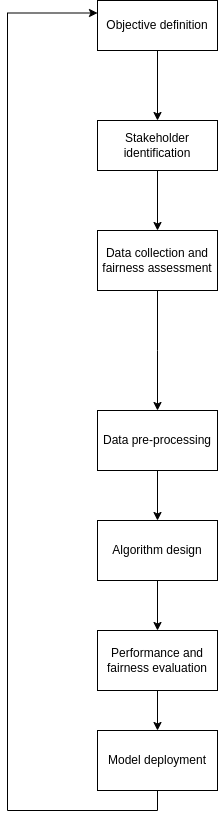
\includegraphics[width=.5\textwidth,height=1\textwidth]{final.png}
    \caption{Fair-by-Design Workflow}
\end{figure}

In the subsequent sections, each of these steps will be comprehensively explored to provide a detailed understanding of the fair-by-design workflow and its ethical underpinnings.

\section{Objective Definition}
\label{section:objective-definition}

The initial step in a fair-by-design workflow involves the precise definition of the system's objectives. Clarity in articulating these objectives is crucial for guiding subsequent design decisions. In the context of fairness, it is essential to explicitly incorporate fairness considerations into the defined objectives.

\subsection{Key Considerations}

\begin{enumerate}

    \item \emph{Clarity and Precision:}

        \begin{itemize}

            \item 
            The specific objectives of the system or process should be defined with clarity and precision to ensure a focused and effective approach. This involves articulating clear and measurable goals that align with the overall purpose of the system. Objectives should avoid ambiguity and provide a concrete understanding of what the system aims to achieve. Clarity in objectives not only guides the development and implementation processes but also facilitates accurate evaluation of the system's success in meeting its intended goals.
            
            \item 
            Clearly articulating the intended functionalities, goals, and expected outcomes is essential for providing a comprehensive understanding of the system or process. Functionalities should be described in detail, outlining the specific tasks or operations the system is designed to perform. Goals should be stated with precision, highlighting the overarching aims that the system seeks to accomplish. Additionally, expected outcomes need to be clearly defined, specifying the anticipated results or benefits that stakeholders can expect from the successful implementation of the system. This clarity ensures alignment between development efforts and the envisioned impact, facilitating effective communication and collaboration among all involved parties.
        
        \end{itemize}
    
    \item \emph{Incorporating Fairness:}

        \begin{itemize}
            
            \item Explicitly stating the importance of fairness in achieving the defined objectives is paramount. Fairness serves as a foundational principle that underpins the ethical and equitable functioning of the system. By ensuring fair treatment of all individuals or groups affected by the system, it enhances trust, mitigates potential biases, and promotes inclusivity. The acknowledgment of fairness as a crucial element in the pursuit of objectives reflects a commitment to ethical practices and responsible deployment. Moreover, it aligns the system with societal values, legal standards, and stakeholder expectations, fostering a positive impact on both the system's performance and its broader social implications.
            
            \item The alignment of fairness with the overall purpose of the system is integral to its effectiveness and societal impact. Fairness ensures that the system operates in a manner that is just, unbiased, and considerate of diverse perspectives. In alignment with the system's purpose, fairness enhances the legitimacy of outcomes, promotes equal opportunities, and guards against discriminatory practices. By incorporating fairness as a core element, the system not only achieves its defined objectives more ethically but also contributes to a more inclusive and equitable societal framework. Fairness becomes a driving force that strengthens the system's purpose, fostering trust and positive engagement among users and stakeholders while minimizing negative consequences and disparities.
        
        \end{itemize}
    
    \item \emph{Balancing Objectives:}

        \begin{itemize}
            
            \item Striking a delicate balance among various objectives is paramount, and it necessitates meticulous consideration to prevent the compromise of fairness in the pursuit of other goals. While the system may have multifaceted objectives such as efficiency, accuracy, and speed, the commitment to fairness should remain unwavering. This balance entails optimizing the system to meet its diverse goals without perpetuating biases or causing harm to specific groups. It requires a nuanced approach, where trade-offs are carefully evaluated to ensure that fairness is not sacrificed for the sake of expediency or efficiency. By upholding fairness as a foundational principle, the system can achieve a harmonious equilibrium, fostering an environment where diverse objectives are met without undermining the ethical considerations embedded in the pursuit of those objectives.
            
            \item Identifying potential conflicts and establishing priorities among competing objectives is a crucial aspect of navigating the complex landscape of system development. Fairness, while paramount, may sometimes appear to conflict with other objectives such as efficiency or cost-effectiveness. In such scenarios, it becomes imperative to conduct a thorough analysis to discern the nature and extent of these conflicts. Establishing clear priorities involves assessing the relative importance of each objective and determining where compromises can be made without compromising the ethical principles underpinning fairness. This process demands a careful weighing of trade-offs, with the ultimate goal of aligning competing objectives in a manner that upholds fairness as a non-negotiable priority while still achieving overall system efficiency and effectiveness.
        
        \end{itemize}

\end{enumerate}

\subsection{Detailed Implementation Steps}

\subsubsection{Stakeholder Engagement}

\begin{itemize}

    \item \emph{Objective:} Engaging key stakeholders, including end-users, developers, and decision-makers, in the definition of objectives is a fundamental step towards fostering a collaborative and inclusive approach to system development. By involving these stakeholders from the outset, their diverse perspectives and insights can be incorporated into the objective-setting process. End-users provide valuable input based on their real-world needs, developers offer technical expertise, and decision-makers contribute strategic considerations. This collective engagement not only ensures a comprehensive understanding of the system's purpose but also enhances the likelihood of creating a solution that aligns with the varied requirements and expectations of all involved parties. It establishes a collaborative foundation that is essential for achieving consensus on objectives and, consequently, for the successful development and implementation of a fair and effective system.

    \item \emph{Implementation:}

        \begin{itemize}
            
            \item Conduct stakeholder interviews, surveys, or workshops to gather insights into their expectations and requirements.
            
            \item Ensure diverse representation to capture a comprehensive range of perspectives.
            
            \item Facilitate open discussions to uncover implicit biases or preferences that may influence objectives.
        
        \end{itemize}

\end{itemize}

\subsubsection{Define Performance Metrics}

\begin{itemize}

    \item \emph{Objective:} Specify the metrics that will be used to measure the success of the system, ensuring a well-defined and quantitative framework for evaluation. These metrics should be carefully selected to align with the established objectives, encompassing both technical performance and fairness considerations. For technical aspects, metrics like accuracy, precision, recall, and F1 score may be relevant, providing insights into the system's overall effectiveness. Simultaneously, metrics such as disparate impact, equalized odds, and overall fairness indices should be included to gauge the system's fairness. The chosen metrics must accurately reflect the intended outcomes and contribute to a comprehensive assessment, enabling a nuanced understanding of the system's success while upholding fairness as a paramount criterion.
    
    \item \emph{Implementation:}
        
    \begin{itemize}
            
        \item Identify traditional performance metrics (e.g., accuracy, precision, recall) relevant to the system's goals.
            
        \item Integrate fairness-specific metrics, such as disparate impact, equalized odds, or statistical parity, depending on the context.
            
        \item Establish a comprehensive set of metrics that collectively address both general system performance and fairness considerations.

    \end{itemize}

\end{itemize}

\subsubsection{Ethical Considerations}

\begin{itemize}

    \item \emph{Objective:} Delve into the ethical implications associated with the defined objectives, conducting a thorough examination to anticipate and address potential ethical challenges. This involves an exploration of how the system's goals and functionalities may intersect with broader ethical considerations, including privacy, security, and societal impact. Consider the implications for different stakeholder groups, ensuring that the system's objectives align with ethical standards and societal values. Articulate clear guidelines and safeguards to mitigate ethical concerns, promoting transparency and accountability throughout the development and implementation phases. By proactively addressing ethical implications, the system can navigate complex ethical landscapes responsibly and contribute to a technology-driven environment that prioritizes ethical considerations alongside technical functionalities.

    \item \emph{Implementation:}

        \begin{itemize}

            \item Conduct an ethical impact assessment to identify potential biases or unintended consequences.

            \item Evaluate the ethical implications of each performance metric, ensuring alignment with fairness goals.

            \item Anticipate scenarios where ethical dilemmas may arise and establish guidelines for resolution.

        \end{itemize}

\end{itemize}

\subsubsection{Documentation}

\begin{itemize}

    \item \emph{Objective:} Thoroughly document the defined objectives in a clear and comprehensive manner, ensuring that each objective is articulated with precision and detail. Provide a detailed overview of the intended functionalities, goals, and expected outcomes, leaving no room for ambiguity. Use concise and unambiguous language to capture the essence of each objective, outlining the specific tasks or functionalities the system aims to achieve. Include any relevant context or background information that enhances the understanding of each objective. This documentation serves as a foundational reference for all stakeholders involved in the development and implementation of the system, fostering a shared understanding of the project's overarching goals and guiding principles. Clarity and comprehensiveness in objective documentation are essential for effective communication and collaboration among team members, end-users, and decision-makers throughout the system's lifecycle.

    \item \emph{Implementation:}

        \begin{itemize}

            \item Create a detailed objective statement that serves as a reference point for all stakeholders.

            \item Document the rationale behind the inclusion of fairness considerations in the objectives.

            \item Maintain a living document that can be updated as objectives evolve or new insights emerge.

        \end{itemize}

\end{itemize}

\subsection{Significance}

Absolutely, defining objectives with precision, incorporating fairness considerations, and establishing clear performance metrics form the foundational pillars of a fair-by-design approach. Precision in objective definition is crucial to avoid ambiguity and guide the development process effectively. Integrating fairness considerations from the outset ensures that ethical principles are not an afterthought but integral to the system's purpose. Clear performance metrics enable the systematic evaluation of the system's success and adherence to fairness goals. Together, these steps create a comprehensive framework that not only aligns the system with ethical standards but also meets stakeholder expectations, fostering trust and accountability throughout the development lifecycle.

\section{Stakeholder Identification}
\label{section:stakeholder-identification}

Engaging key stakeholders is a foundational step in shaping the objectives of a fair-by-design workflow. Stakeholders, representing diverse perspectives and interests, bring invaluable insights that contribute to defining the system's purpose. Involving a range of stakeholders ensures a comprehensive understanding of ethical implications and societal expectations. This inclusive approach not only fosters a sense of collective responsibility but also helps in addressing potential biases and concerns early in the design process. By incorporating various viewpoints, the fair-by-design workflow becomes more attuned to the needs of different communities and stakeholders, enhancing the overall fairness and effectiveness of the system.

\subsection{Key Considerations}

\begin{enumerate}

    \item \emph{Diverse Representation:}

        \begin{itemize}

            \item Ensuring the inclusion of stakeholders who represent a diverse range of perspectives is paramount in the fair-by-design approach. This encompasses stakeholders such as end-users, developers, decision-makers, and members of affected communities. Each stakeholder group contributes unique insights and experiences that are crucial for shaping a system that is equitable and aligned with ethical principles. End-users provide practical insights into how the system will be experienced, developers offer technical expertise, decision-makers provide strategic guidance, and affected communities bring perspectives on potential societal impacts. By actively involving this diverse set of stakeholders, the fair-by-design workflow gains a more holistic understanding of potential biases, ethical considerations, and the broader societal context, ultimately leading to a more inclusive and equitable outcome.
        
        \end{itemize}
    
    \item \emph{Inclusive Decision-Making:}
        
    \begin{itemize}
    
        \item Fostering an inclusive environment is integral to the fair-by-design approach, ensuring that stakeholders actively participate in decision-making processes related to the system's objectives. This inclusivity encourages diverse perspectives, fostering a collaborative atmosphere where each stakeholder's input is valued. Establishing open channels of communication and providing opportunities for meaningful engagement empowers stakeholders to contribute their insights effectively. By creating an inclusive space, the fair-by-design workflow not only captures a broader range of perspectives but also cultivates a sense of ownership among stakeholders. This collaborative decision-making process enhances transparency, builds trust, and ultimately results in a system that is more responsive to the needs and values of the varied stakeholders involved.
    
    \end{itemize}
    
    \item \emph{Transparent Communication:}
    
    \begin{itemize}
    
        \item Maintaining transparent communication channels is crucial in the fair-by-design approach to keep stakeholders informed about the development process and gather their input effectively. Transparent communication fosters trust and ensures that stakeholders are aware of the system's progress, objectives, and any potential implications. Regular updates, clear documentation, and accessible information contribute to an open dialogue, allowing stakeholders to stay engaged and provide valuable feedback. This proactive approach to communication not only enhances the collaborative decision-making process but also promotes a shared understanding of the ethical considerations embedded in the system. Transparent communication channels are a cornerstone of the fair-by-design workflow, fostering a sense of inclusivity and shared responsibility among all stakeholders involved.
    
    \end{itemize}

\end{enumerate}

\subsection{Detailed Implementation Steps}

\subsubsection{Stakeholder Mapping}

\begin{itemize}
    
    \item \emph{Objective:} Identifying and mapping key stakeholders is a crucial step in the fair-by-design approach to understand and incorporate diverse perspectives in the system's development. Key stakeholders include end-users, developers, decision-makers, and affected communities, each bringing unique insights and interests to the table. End-users provide valuable feedback based on their experiences and expectations, guiding user-centric design. Developers contribute technical expertise, ensuring the feasibility and efficiency of the system. Decision-makers offer strategic input aligning the system with broader organizational goals. Affected communities bring a contextual understanding of societal impacts, helping navigate ethical considerations. By mapping these stakeholders, the fair-by-design workflow ensures a holistic and inclusive approach, considering the varied interests and perspectives that shape the system's objectives and ethical considerations.
    
    \item \emph{Implementation:}
    
    \begin{itemize}
    
        \item Create a stakeholder map that identifies different stakeholder groups and their respective roles and interests.
    
        \item Prioritize stakeholders based on their influence on or impact from the system.
    
    \end{itemize}

\end{itemize}

\subsubsection{Engagement Strategies}

\begin{itemize}

    \item \emph{Objective:} Developing effective strategies for stakeholder engagement in the objective-setting process is pivotal for a fair-by-design workflow. Begin by conducting stakeholder analysis to identify key individuals and groups. Establish clear communication channels to disseminate information and gather feedback. Organize workshops, focus groups, or collaborative sessions to facilitate active participation. Tailor engagement methods to suit diverse stakeholders, ensuring inclusivity. Provide accessible documentation outlining the proposed objectives and ethical considerations. Emphasize the value of each stakeholder's input and foster an open dialogue to address concerns. Regularly update stakeholders on the progress, incorporating their feedback iteratively. By employing these strategies, a fair-by-design workflow ensures comprehensive engagement, enriching the objective-setting process with diverse perspectives and reinforcing ethical considerations.

    \item \emph{Implementation:}

    \begin{itemize}

        \item Tailor engagement strategies to the characteristics of each stakeholder group (e.g., workshops, surveys, focus groups).

        \item Clearly communicate the importance of their input in shaping the ethical foundations of the system.

    \end{itemize}

\end{itemize}

\subsubsection{Inclusive Workshops or Meetings}

\begin{itemize}

    \item \emph{Objective:} In fostering an inclusive fair-by-design approach, organizing workshops or meetings is instrumental for stakeholder engagement in defining objectives. These sessions provide a platform for active participation, allowing diverse stakeholders, including end-users, developers, decision-makers, and affected communities, to contribute insights. The workshops should be designed to encourage open dialogue, ensuring that each perspective is heard and considered. Employ facilitation techniques that promote inclusivity, such as structured discussions, brainstorming sessions, or collaborative activities. By facilitating these inclusive workshops, the fair-by-design workflow embraces diverse viewpoints, enriching the objective-setting process and reinforcing its commitment to ethical considerations.

    \item \emph{Implementation:}

    \begin{itemize}

        \item Organize collaborative sessions that encourage open dialogue and the exchange of diverse perspectives.

        \item Provide a platform for stakeholders to express their values, concerns, and expectations related to fairness in the system.

    \end{itemize}

\end{itemize}

\subsubsection{Feedback Collection}

\begin{itemize}

    \item \emph{Objective:} After defining initial objectives and ethical considerations in the fair-by-design workflow, it is crucial to gather feedback from stakeholders. Establish a feedback loop through surveys, interviews, or focus group discussions to ensure that the proposed objectives resonate with the diverse perspectives of stakeholders. This iterative process allows for refinements and adjustments based on the input received. Actively seeking feedback fosters collaboration and ensures that the fair-by-design approach remains responsive to the evolving needs and expectations of stakeholders throughout the system's development.

    \item \emph{Implementation:}

    \begin{itemize}

        \item Utilize surveys, interviews, or online platforms to collect structured feedback.

        \item Encourage stakeholders to provide qualitative insights that may not be captured by quantitative methods.

    \end{itemize}

\end{itemize}

\subsection{Significance}

Stakeholder identification is a pivotal aspect of ensuring the fair and inclusive development of a system. Involving stakeholders from diverse backgrounds and perspectives allows the ethical considerations embedded in the objectives to more accurately reflect the values and expectations of the broader community. By recognizing and engaging with a variety of stakeholders, including end-users, developers, decision-makers, and representatives from affected communities, the fair-by-design approach becomes more comprehensive and responsive to the multifaceted needs and concerns of the people who will interact with or be impacted by the system. This inclusive process contributes to the development of a system that is not only technically sound but also ethically grounded and considerate of various societal perspectives.

\section{Data Collection: Integration with Stakeholder Considerations}
\label{section:data-collection}

In the process of data collection, the integration of insights from stakeholders is crucial, particularly for the identification of protected attributes. Stakeholders bring valuable perspectives on societal norms, ethical considerations, and potential biases that may not be apparent solely from the dataset. Their input aids in defining and recognizing protected attributes, contributing to a more nuanced understanding of fairness in the context of the application.

\subsection{Importance of Stakeholder Integration}

\subsubsection{Cultural Sensitivity}


Stakeholders, representing diverse backgrounds, contribute significantly to a nuanced understanding of cultural norms and sensitivities within the fair-by-design approach. This diversity is crucial in recognizing attributes that may be culturally significant and warrant protection. For instance, certain cultural or religious practices may involve sensitive information that should be identified as a protected attribute to ensure respectful and unbiased treatment. By actively involving stakeholders who bring a range of cultural perspectives, the objective-setting process can identify and address potential biases associated with cultural attributes, fostering a system that respects and reflects the rich diversity of its user base. This approach not only enhances fairness but also promotes cultural sensitivity and inclusivity in the design and implementation of the system.

\subsubsection{Contextual Relevance}


Stakeholders play a crucial role in providing contextual insights that may not be evident in the dataset alone within the fair-by-design approach. Their considerations can guide the identification of attributes relevant to the specific application and its ethical implications. For instance, in an educational context, stakeholders might highlight attributes related to socio-economic status or learning styles that could impact fairness considerations in student evaluations. By actively involving stakeholders, the objective-setting process gains valuable perspectives that enrich the ethical framework of the system. This collaborative approach ensures that the identified objectives not only align with technical requirements but also address real-world considerations, promoting a more holistic and socially responsible system.

\subsubsection{Uncovering Implicit Biases}

Stakeholders play a crucial role in uncovering implicit biases that may not be explicitly represented in the dataset within the fair-by-design approach. By incorporating their perspectives, the identification of protected attributes becomes more comprehensive and reflective of potential sources of bias. This is particularly important in domains where historical biases or societal prejudices might influence decision-making processes. Stakeholders can provide valuable input to address and mitigate these implicit biases, contributing to the development of a more equitable and unbiased system. Their involvement ensures a thorough examination of potential biases, fostering transparency and fairness in the system's design and objectives.

\subsection{Implementation Steps}

\subsubsection{Stakeholder Workshops}

\emph{Objective:} Integrate stakeholder considerations into the identification of protected attributes.

\emph{Implementation:}

\begin{itemize}

    \item Conduct stakeholder workshops specifically focused on discussing and identifying potential protected attributes.

    \item Encourage open discussions to uncover implicit biases or attributes that may have societal implications.

    \item Facilitate collaboration between data scientists and stakeholders to ensure a shared understanding of fairness goals.

\end{itemize}

\subsubsection{Documentation of Stakeholder Input}

\emph{Objective:} Document stakeholder input on protected attributes for transparency.

\emph{Implementation:}

\begin{itemize}

    \item Record the insights shared by stakeholders regarding attributes they perceive as sensitive or requiring protection.

    \item Incorporate stakeholder considerations into the broader documentation of the data collection process.

    \item Provide clear documentation of the integration process to maintain transparency and facilitate reproducibility.

\end{itemize}

\subsection{Assessing Fairness: Disparate Impact Metric}

In order to assess the fairness of the dataset over the protected attributes identified with stakeholders, the disparate impact metric is commonly employed. The disparate impact metric quantifies the difference in outcomes between different groups, highlighting potential disparities in how the dataset represents protected attributes.

\subsubsection{Application}

\begin{itemize}
    
    \item Calculate the disparate impact for each identified protected attribute to evaluate the potential disparities in the dataset.
    
    \item Establish a baseline value for disparate impact, considering fairness thresholds and legal requirements.

\end{itemize}

\subsubsection{Significance}

The disparate impact metric serves as a quantitative tool to gauge the fairness of the dataset over identified protected attributes. Its application allows data scientists to identify and address potential biases in the data collection process, contributing to a more equitable foundation for subsequent stages in the fair-by-design workflow.

\section{Data Pre-processing}
\label{section:pre-proc}

After the data collection and integration of stakeholder considerations, the next crucial stage is data pre-processing. This stage focuses on preparing and cleaning the dataset to address biases, imbalances, and ensure fairness in subsequent stages of the fair-by-design workflow.

\subsection{Key Considerations}

\begin{enumerate}

    \item \emph{Data cleaning:} 

    This process involves identifying and rectifying errors, inconsistencies, and inaccuracies in the raw dataset to ensure its reliability and quality. Common tasks in data cleaning include handling missing values, correcting data format issues, removing duplicates, and addressing outliers. The goal is to create a clean, standardized dataset that forms a solid foundation for subsequent analysis and model development. Rigorous data cleaning is essential for mitigating the risk of biased or inaccurate model outcomes, as machine learning models heavily depend on the quality of the input data. This meticulous attention to data quality sets the stage for effective feature engineering, model training, and, ultimately, the generation of reliable and fair predictions.

    \item \emph{Handling Protected Attributes:} 
    
    Within the Fair-by-Design workflow, a meticulous transformation process is applied to protected attributes, assumed to be categorical in nature. This transformative step is pivotal for ensuring fairness in subsequent stages of the machine learning pipeline, aiming to mitigate potential biases associated with these attributes and foster equitable treatment within the model.

    The transformation process for categorical protected attributes involves the identification of the most frequent value and the subsequent application of a binary encoding scheme. This nuanced procedure plays a crucial role in aligning the dataset with the fairness objectives of the Fair-by-Design workflow.

    Let $P$ be the set of protected attributes, and $p_i$ represent a specific protected attribute within $P$. The most frequent value, denoted as $v_{\text{freq}}$, is determined for each categorical protected attribute $p_i$ in the dataset through the following formalism:

    \[
    v_{\text{freq}} = \text{argmax}_v \left( \text{count}(p_i = v) \right)
    \]
    
    This calculation ensures a comprehensive understanding of the prevalent categories within these attributes.

    The binary representation preserves the essential information about protected attributes, providing a condensed yet informative encoding that reflects the privilege or lack thereof concerning specific attributes.

    During the training phase, the model learns to distinguish instances based on privilege or lack thereof concerning specific attributes, as represented by the binary encoding. This facilitates effective model incorporation and decision-making during training and prediction phases.

    This nuanced encoding strategy serves as the foundation for unbiased and fair treatment of instances within the model. By transforming categorical protected attributes into a binary representation, the Fair-by-Design workflow ensures that subsequent machine learning models can effectively incorporate and act upon this information during training and prediction phases, contributing significantly to the development of a more equitable and ethically sound machine learning model.

    \item \emph{Handling Output Variable:} 
    
    The handling of the output variable in the Fair-by-Design workflow is a nuanced process that adapts to the nature of the variable, whether categorical or continuous. This tailored treatment is essential for aligning the prediction task with the fairness objectives of the workflow, ensuring that the model's predictions are not only accurate but also ethically sound.


    In cases where the output variable is categorical, the workflow initiates by determining the most frequent value within this category. Let $Y$ represent the output variable, and $y_i$ be a specific outcome within $Y$. The most frequent value, denoted as $y_{\text{freq}}$, is determined through the following formalism:

    \[
    y_{\text{freq}} = \text{argmax}_y \left( \text{count}(Y = y) \right)
    \]

    This strategic calculation provides insights into the prevailing outcome within the dataset. Subsequently, instances where the output variable matches $y_{\text{freq}}$ are replaced with the binary representation 1, while all other instances take on the binary representation 0. The binary encoding function is defined as follows:

    \[
    \text{Binary Encoding}(y_i) = \begin{cases} 
    1 & \text{if } y_i = y_{\text{freq}} \\ 
    0 & \text{otherwise}
    \end{cases}
    \]

    This transformation effectively redefines the prediction task, shifting the focus to discerning whether a given sample belongs to the most frequent outcome. The binary encoding approach not only simplifies the representation of categorical outcomes but also enables the model to make predictions in a manner that aligns with fairness considerations.


    Conversely, when the output variable is continuous, the workflow employs a distinct strategy. Let $Z$ represent the continuous output variable, and $z_i$ be a specific value within $Z$. Values of the continuous variable that surpass the mean are replaced with 1, while those falling below the mean assume the binary representation 0. This adjustment transforms the prediction task into establishing whether a sample's continuous output is above the mean. The binary encoding function for continuous variables is defined as:

    \[
    \text{Binary Encoding}(z_i) = \begin{cases} 
    1 & \text{if } z_i > \text{mean}(Z) \\ 
    0 & \text{otherwise}
    \end{cases}
    \]

    This approach ensures that the model is not only attentive to the central tendency of the continuous variable but also considers the distribution of values concerning the mean.

    This tailored and meticulous treatment of the output variable underscores the commitment of the Fair-by-Design workflow to equitable and ethical machine learning practices. The workflow not only adapts to the inherent characteristics of the data but also ensures that the subsequent model operates with a heightened awareness of fairness considerations, contributing to the development of a more responsible and unbiased machine learning model.

\end{enumerate}

This nuanced pre-processing step sets the groundwork for a fair and unbiased learning prediction, aligning the dataset with the ethical considerations embedded in the Fair-by-Design workflow.

\section{Algorithm Design}
\label{section: algorithm-design}

The Algorithm Design stage in the fair-by-design workflow is a critical phase where machine learning models are chosen, adapted, or developed to align with the defined objectives and fairness considerations. The overarching goal is to design models that not only achieve high accuracy but also adhere to ethical and fair principles. This section provides a detailed exploration of the key considerations, strategies, and implementation steps involved in Algorithm Design.

\subsection{Key Considerations}

\begin{enumerate}

    \item \emph{Fairness-Aware Model Selection:} 
    
    The choice of machine learning models plays a pivotal role in achieving fairness objectives. Fairness-aware model selection involves considering models that have built-in mechanisms to address biases and promote equitable outcomes. Models such as adversarial networks, fairness-aware classifiers, and re-weighted learning algorithms are commonly explored.

    \item \emph{Regularization Techniques:} 
    
    Regularization methods, such as demographic parity constraints or equalized odds constraints, are employed to guide the model toward fair predictions. These techniques add fairness constraints to the optimization process, promoting equitable outcomes across different demographic groups.

    \item \emph{Bias Detection and Mitigation:} 
    
    Embedding mechanisms for detecting and mitigating biases within the algorithm is essential. This involves continuous monitoring of the model's predictions for disparate impact and implementing corrective measures to mitigate biases as they emerge.

    \item \emph{Pre-processing, In-processing, or Post-processing Algorithms:} 
    
    The selection of pre-processing, in-processing, or post-processing algorithms is a strategic decision influenced by the specific characteristics of the data and fairness goals. Pre-processing algorithms transform the dataset before model training, in-processing algorithms modify the learning process, and post-processing algorithms adjust predictions after model training. Consider the nature of biases, the available data, and the desired level of fairness when choosing the appropriate approach.

\end{enumerate}

\subsection{Detailed Implementation Steps}

% Include the detailed implementation steps for each key consideration as per the previous discussion.

\subsubsection{Fairness-Aware Model Selection}

\begin{itemize}

    \item \emph{Exploration of Fairness-Aware Models:}
     
    \begin{itemize}
    
        \item In the pursuit of developing a fair-by-design machine learning model, a crucial step involves conducting a comprehensive survey and evaluation of existing fairness-aware models that are tailored to the specific application domain. This process entails a thorough examination of the literature and available models, considering their performance, interpretability, and fairness considerations. By evaluating existing models, practitioners gain valuable insights into the strengths and limitations of different approaches, allowing them to make informed decisions about the most suitable model for their specific use case. This diligent survey and evaluation contribute to the foundation of a fair-by-design workflow, ensuring that the chosen model aligns with both technical requirements and ethical considerations inherent to the application domain.
    
        \item When exploring fairness-aware models for a specific application domain, it is prudent to consider models that explicitly address bias. This includes but is not limited to adversarial networks or models with built-in fairness constraints. Adversarial networks are designed to mitigate bias by introducing a secondary network that works to identify and counteract any discriminatory patterns in the primary model. On the other hand, models with built-in fairness constraints incorporate predefined fairness metrics into the optimization process, ensuring that the model adheres to fairness criteria during training. Evaluating these specialized models provides a nuanced understanding of their efficacy in handling bias, offering practitioners valuable insights into the most suitable approach for mitigating bias within their specific context. This consideration reinforces the fair-by-design approach, emphasizing the importance of selecting models that actively address and rectify biases to promote equitable outcomes in machine learning applications.
    
    \end{itemize}
    
    \item \emph{Implementation and Customization:}
    
    \begin{itemize}
    
        \item Once a fairness-aware model is chosen for the specific application domain, the next step is to implement it in the selected machine learning framework. This involves translating the model specifications and architecture into code, configuring the necessary parameters, and integrating it seamlessly into the overall machine learning pipeline. The implementation process should adhere to best practices and guidelines provided by the chosen framework, ensuring optimal performance and compatibility. Additionally, developers need to consider the interpretability of the model, as transparency is crucial in understanding how fairness considerations are embedded within the system. The successful implementation of the fairness-aware model marks a pivotal stage in the fair-by-design workflow, laying the foundation for subsequent training, evaluation, and deployment phases with a heightened commitment to equitable and unbiased machine learning outcomes.
    
        \item After implementing the selected fairness-aware model, it's crucial to customize the model to align with the unique characteristics of the dataset and the specific fairness objectives defined earlier in the workflow. This customization involves fine-tuning model parameters, adjusting hyperparameters, and incorporating features that account for the nuances present in the dataset. Additionally, developers may need to introduce specific fairness-oriented adjustments to the model architecture, ensuring that it can effectively handle and mitigate biases associated with protected attributes. This tailored customization is essential for maximizing the model's performance within the context of the fair-by-design approach, where the goal is not only technical excellence but also ethical and unbiased machine learning outcomes.
    
    \end{itemize}

\end{itemize}

\subsubsection{Explainability and Interpretability}

\begin{itemize}

    \item \emph{Model Selection:}

    \begin{itemize}

        \item In the fair-by-design workflow, selecting models known for their high explainability and interpretability is a strategic choice. Decision trees and rule-based models, renowned for their transparency, are preferred in this context. The rationale behind this selection is rooted in the commitment to transparency and accountability. Models that are easily interpretable enable stakeholders, including end-users and decision-makers, to understand the decision-making process. This transparency not only fosters trust but also allows for the identification and mitigation of any potential biases or fairness concerns. By opting for models with high explainability, the fair-by-design workflow aligns with its overarching goal of developing machine learning systems that are not only technically robust but also ethically sound and easily understandable by a diverse range of stakeholders.

        \item When integrating fairness considerations into model selection within the fair-by-design workflow, it's crucial to carefully weigh the trade-offs between model complexity and interpretability. The specific application requirements play a pivotal role in determining the optimal balance. While highly complex models might offer superior predictive performance, they often sacrifice interpretability. On the other hand, interpretable models, such as decision trees or rule-based models, may have limitations in capturing intricate patterns present in the data. Striking the right balance is essential; the fair-by-design approach aims to ensure not only fairness but also transparency. Therefore, selecting models that align with the interpretability needs of stakeholders while still meeting the performance requirements is a key consideration in the design process. This conscious decision-making contributes to the development of fair, understandable, and accountable machine learning models.

    \end{itemize}

\end{itemize}

\subsubsection{Regularization Techniques}

\begin{itemize}

    \item \emph{Integration of Fairness Constraints:}

    \begin{itemize}

        \item The integration of fairness constraints requires a nuanced understanding of the specific fairness goals and metrics relevant to the application domain. The fair-by-design approach emphasizes a principled and systematic incorporation of these constraints to mitigate biases and promote equitable outcomes. By embedding fairness into the training process, the workflow aims to foster models that not only deliver accurate predictions but also adhere to ethical and fairness considerations, contributing to responsible and unbiased machine learning practices

        \item Experimenting with different regularization techniques is a crucial aspect of the fair-by-design approach to machine learning. Regularization methods, such as demographic parity constraints or equalized odds constraints, play a significant role in mitigating biases and promoting fairness within models. These techniques are tailored to address specific fairness considerations related to protected attributes, ensuring that the model's predictions are not unduly influenced by factors like gender, race, or other sensitive attributes.

    \end{itemize}

\end{itemize}

\subsubsection{Bias Detection and Mitigation}

\begin{itemize}
    
    \item \emph{Dynamic Bias Mitigation:}
    
    \begin{itemize}
    
        \item Developing adaptive algorithms that dynamically adjust to emerging biases in the data is a proactive strategy within the fair-by-design framework. These algorithms are designed to continuously monitor and evaluate the model's performance, identifying any potential biases that may arise during operation. The adaptive nature of these algorithms allows them to dynamically adjust their parameters or decision boundaries to mitigate the impact of emerging biases, ensuring ongoing fairness in real-world applications.
    
        \item Implementing corrective measures, such as re-weighting or re-sampling, is a pivotal step in the fair-by-design workflow to actively mitigate biases as they are detected. When biases are identified through ongoing monitoring, these corrective measures are strategically applied to address the imbalances and promote fairness in the model's predictions.
    
    \end{itemize}

\end{itemize}

\subsubsection{Human-in-the-Loop Approaches}

\begin{itemize}
    
    \item \emph{Stakeholder Collaboration:}
    
    \begin{itemize}
    
        \item Facilitate collaboration sessions with domain experts and stakeholders to understand fairness nuances.
    
        \item Involve stakeholders in model validation and decision-making processes.
    
    \end{itemize}

\end{itemize}

\subsection{Pre-processing Algorithms Proposed}

\subsubsection{Fairness through data rebalancing}
\label{subsec:ftdr}

In this approach, the paradigm of bias mitigation takes on a unique and innovative perspective, one that prioritizes data augmentation over attribute removal. Unlike traditional approaches that center on the exclusion of specific attributes, this methodology embraces the concept of data augmentation, introducing a distinctive definition of fairness and equity within the AI system.

The essence of this approach revolves around the augmentation of the dataset by introducing new data instances that offer a more comprehensive and inclusive representation of the underlying population. This expanded dataset is designed to be more diverse, representative, and balanced, transcending the limitations of the original data and fostering a more nuanced understanding of fairness. 

The introduction of augmented data instances leads to a redefined notion of fairness within the AI system. Instead of solely focusing on the absence of biased attributes, fairness is now measured in terms of the dataset's inclusivity and its ability to capture the diversity and nuances present within the population it seeks to serve. 

This approach aligns with the broader philosophy of ensuring that AI systems are equitable, just, and capable of making informed and unbiased decisions. By augmenting the dataset, it strives to bridge the gaps in representation and provide a more equitable playing field for all individuals, regardless of their background or characteristics. 

The process of data augmentation necessitates a careful selection of techniques and methodologies that can introduce new data instances while maintaining the integrity and quality of the dataset. These techniques may encompass oversampling, synthetic data generation, or other data synthesis methods, each tailored to the specific context and objectives of the AI system.

In traditional fairness definitions, the focus often revolves around ensuring fair treatment for individual protected attributes, denoted as $A_1, A_2, \ldots, A_k$. While this is undoubtedly crucial, a more comprehensive understanding of fairness calls for an examination of fairness in the context of combinations of protected attributes and the output. A new definition of fairness is proposed, which takes into account the representation of all combinations of $k$ protected attributes and the output, aiming for equitable representation across these combinations.

A fair dataset is defined as one in which, for each combination of protected attributes $\{A_1, A_2, \ldots, A_k\}$ and the output $O_j$, the representation is equal and proportional. Mathematically, a dataset is fair if:

\[
\forall i_1, i_2, \ldots, i_k, j: \frac{|D_{i_1, i_2, \ldots, i_k, j}|}{|D|} = \text{constant}
\]

where:
- $D$ is the dataset,
- $|D_{i_1, i_2, \ldots, i_k, j}|$ is the number of samples with the specific combination of protected attributes $A_{i_1}, A_{i_2}, \ldots, A_{i_k}$ and output $O_j$,
- $|D|$ is the total number of samples in the dataset.

This entails that any combination of demographic groups, defined by the protected attributes, and the output should have comparable representation, thereby fostering a balanced and unbiased dataset.

By striving for equal representation of combinations of protected attributes, is addressed a fundamental aspect of fairness that transcends individual attributes. This approach provides a more nuanced understanding of fairness by considering the intersections of various demographic groups. It encourages a broader examination of potential biases that may arise when considering multiple attributes simultaneously.

Incorporating this definition of fairness into the dataset rebalancing process enables us to promote a comprehensive notion of fairness, aligning with the principles of equal opportunity and non-discrimination across all combinations of protected attributes. Our subsequent algorithm and experimental evaluation are designed to actualize this definition and demonstrate its effectiveness in achieving a more equitable representation within the dataset.

At this point it's necessary to begin with a formalization for the algorithm itself.


Let \( D \) be a dataset \( R^{n \times m} \), where \( n \) is the number of samples and \( m \) is the number of features. Let \( k \) be the number of protected variables represented as \( R^{n \times 1} \), and let there be a single output variable represented as \( R^{n \times 1} \).

A rebalancing function \( \mathcal{R} \) can be formally defined as a mapping:

\[
\mathcal{R}: R^{n \times m} \rightarrow R^{l \times m}
\]

where \( l > m \), and the function \( \mathcal{R} \) transforms the input dataset \( D \) of dimensions \( n \times m \) into an output dataset \( D' \) of dimensions \( l \times m \).



Let \( k \) be the number of binary protected variables in the dataset \( D \), and consider the output variable to be binary as well. The number of possible combinations of these variables is \( 2^{(k+1)} \).

Consider a set \( \text{Combination-frequency} \) with occurrences of all \( 2^{(k+1)} \) combinations within the dataset. For each combination, the number of rows in which that combination appears should be equal to the maximum occurrence among all combinations present in the set \( \text{Combination\textunderscore frequency} \). This maximum value is denoted as \( \text{Max}(\text{Combination-frequency}) \).

Mathematically, the number of rows (\( l \)) the final dataset should have for each combination is given by:

\[
l = \text{Max}(\text{Combination-frequency})
\]



Let \( l \) be the desired number of rows for the final dataset. For each combination of values, is calculated the occurrence count \( \text{occurrence}_i \), where \( i \) ranges from 1 to \( 2^{(k+1)} \), with \( k \) being the number of protected binary variables and considering the output variable as binary.

The total number of rows to be added is given by:

\[
\text{total\_rows\_to\_add} = l - \sum_{i=1}^{2^{(k+1)}} \text{occurrence}_i
\]

For each iteration:

\begin{itemize}

    \item The values of the protected and output variables are set according to the specific combination.
    
    \item For all other attributes, a random value \( \text{random\_value}_{ij} \) is generated, where \( j \) represents the specific attribute and \( i \) represents the row being added for that attribute. \( \text{random\_value}_{ij} \) is within the minimum and maximum range for attribute \( j \).

\end{itemize}

As showed in the following pseudocode

\begin{algorithm}[H]
    \caption{Reabalancing}
    \begin{algorithmic}[1]
        \State \textbf{Input:} combination\_set, combination\_frequency, protected\_attributes, dataset\_attributes
        \State \textbf{Output:} Updated dataset

        \State max\_frequency $\gets$ max(combination\_frequency)

        \For{index \textbf{in} (0, len(combination\_set) - 1)}
            \State combination $\gets$ combination\_set[index]
            \State frequency $\gets$ combination\_frequency[index]
            \State combination\_dataset $\gets$ dataset[dataset[combination] == combination\_set[index]]

            \While{frequency $<$ max\_frequency}
                \State new\_row $\gets$ empty

                \For{(attr, val) \textbf{in} (combination, protected\_attributes)}
                    \State new\_row[attr] $\gets$ val
                \EndFor

                \For{attr \textbf{in} dataset\_attributes \textbf{and not in} protected\_attributes}
                    \State new\_row[attr] $\gets$ random(min(combination\_dataset[attr]), max(combination\_dataset[attr]))
                \EndFor

                \State dataset.add(new\_row)
                \State frequency $+$= 1
            \EndWhile
        \EndFor

        \State \textbf{return} Updated dataset
    \end{algorithmic}
\end{algorithm}

this algorithm adds rows to the dataset until every combination have the same frequency. Fundamental for this algorithm is the way in which are generate the value for the variables not involved into the combination. These are added considering the sub-dataset of the original dataset in which the combination occurs. 


\subsection{Significance}

The Algorithm Design stage is pivotal in shaping the ethical and fair behavior of machine learning models within the fair-by-design framework. By carefully selecting, customizing, and integrating fairness-aware models, and incorporating transparency and human-in-the-loop approaches, this stage ensures that the resulting models align with ethical considerations and promote equitable outcomes.

\section{Model Training and Evaluation}
\label{section:model-training}

\subsection{Introduction}

This section provides a comprehensive account of the model training and evaluation process within the Fair-by-Design framework. Following the meticulous application of the selected pre-processing, in-processing, or post-processing algorithm, the training phase becomes pivotal for crafting a machine learning model that aligns not only with accuracy objectives but also with the ethical considerations of fairness.

\subsection{Training Process}

\subsubsection{Data Splitting}

The dataset undergoes a thoughtful split into training, validation, and test sets. This division serves a strategic purpose: the training set propels the model's learning, the validation set aids in hyperparameter tuning to enhance generalization, and the test set evaluates the final model's performance, providing a reliable measure of its predictive capabilities.

\subsubsection{Model Architecture}

The architecture of the chosen model is crafted with a delicate balance between accuracy and fairness considerations. Architectures may include innovative components, such as adversarial layers or customized modules designed to enforce fairness constraints. The emphasis is on creating a model that is not only proficient in capturing complex patterns but also interpretable and transparent in its decision-making.

\subsubsection{Training Parameters}

Key training parameters, including the learning rate, batch size, and convergence criteria, are meticulously tuned. The learning rate dictates the step size in the optimization process, influencing the rate of model parameter updates. The batch size determines the number of samples processed in each iteration, impacting the efficiency and resource utilization. Convergence criteria ensure that the training process halts when the model reaches optimal performance, preventing overfitting.

\subsubsection{Fairness Constraints (if applicable)}

In scenarios where fairness constraints are integrated into the training process, they are defined and enforced. This may involve the introduction of regularization terms designed to penalize disparate treatment of different demographic groups. Adversarial training components might also be employed to mitigate bias and promote equitable outcomes.

\subsubsection{Model Training}

The model undergoes training for a predetermined number of epochs. Leveraging the training set, the model iteratively updates its parameters to minimize the loss function. This iterative process aims at achieving a balance between accuracy and fairness, contributing to the development of a machine learning model that is not only adept at capturing underlying patterns but also conscious of potential biases.

\subsection{Evaluation Metrics}

\subsubsection{Accuracy Metrics}

A suite of accuracy metrics is employed to holistically assess the model's overall performance:

\begin{itemize}
    \item \emph{Accuracy:} The ratio of correctly predicted instances to the total instances.
    
    \item \emph{Precision:} The proportion of true positive predictions among instances predicted as positive.
    
    \item \emph{Recall:} The proportion of true positive predictions among actual positive instances.
    
    \item \emph{F1-score:} The harmonic mean of precision and recall, providing a balanced measure of accuracy.
\end{itemize}

\subsubsection{Fairness Metrics}

Fairness metrics are instrumental in evaluating the model's behavior across different demographic groups:

\begin{itemize}
    
    \item \emph{Equalized Odds:} Evaluates whether the model provides similar false positive and false negative rates across different demographic groups.
    
    \item \emph{Statistical Parity:} Examines the proportion of positive outcomes for each demographic group to identify disparities.
\end{itemize}

\subsection{Results and Analysis}

\subsubsection{Accuracy Results}

A meticulous analysis of accuracy results provides valuable insights into how well the model predicts the target variable. Precision, recall, and F1-score metrics offer a nuanced understanding of the trade-offs between true positives, false positives, and false negatives. The goal is not just accuracy but a balanced and informed prediction capability.

\subsubsection{Fairness Results}

Fairness metrics serve as a critical lens to identify and address biases within the model. Disparate impact, equalized odds, and statistical parity results are analyzed to assess whether the model exhibits disparate treatment of different demographic groups. The focus is on identifying and mitigating disparities, fostering a model that is fair and equitable.

\subsubsection{Trade-offs}

Understanding the trade-offs between accuracy and fairness is vital. In pursuit of a balanced model, adjustments may be necessary. Techniques such as re-weighting, re-sampling, or customized loss functions may be employed to address specific fairness concerns. Striking the right balance becomes a central theme in refining the model for optimal performance.

\subsection{Discussion}

\subsubsection{Interpretability}

The interpretability of the model's decisions is paramount. Techniques such as SHAP (SHapley Additive exPlanations) values or LIME (Local Interpretable Model-agnostic Explanations) are explored to enhance transparency in the decision-making process. Understanding how the model arrives at its predictions contributes to the model's trustworthiness.

\subsubsection{Ethical Considerations}

The discussion extends to ethical considerations arising from the model's behavior. Attention is given to potential biases, unintended consequences, and the impact on different demographic groups. Strategies for addressing ethical concerns are proposed, underscoring the commitment to responsible and ethical AI practices.

\subsubsection{Further Refinement}

Based on the observed results, proposals for further refinement are put forth. This may involve adjusting fairness constraints, fine-tuning hyperparameters, or exploring alternative algorithms to enhance both accuracy and fairness in model predictions. The iterative nature of this refinement process reflects the commitment to continuous improvement and the pursuit of fair

\section{Model Deployment}
\label{section:model-deployment}

\subsection{Introduction}

Model deployment is a critical phase in the fair-by-design framework, where the fair machine learning model transitions from development to practical application in real-world decision-making processes. This phase emphasizes the integration of the model into decision systems, ongoing monitoring to ensure fairness, user education, and iterative refinement based on feedback.

\subsection{Integration with Decision Systems}

The seamless integration of the fair machine learning model into decision systems is guided by the principles of fairness and ethical AI practices. Attention is given to the alignment of the model with existing infrastructure, ensuring that its predictions contribute meaningfully to decision-making processes. This integration involves a careful consideration of potential biases and fairness implications at every stage of the decision-making pipeline.

\subsection{Monitoring and Feedback Loops}

A robust monitoring system is established to continuously evaluate the model's performance in real-world scenarios. This monitoring process extends beyond traditional accuracy metrics, placing a specific focus on fairness indicators. Feedback loops are implemented to capture any deviations from fairness objectives, changes in the data distribution, or emerging ethical considerations.

User feedback becomes a crucial component of the monitoring process. Users interacting with the model contribute valuable insights into its real-world impact. The feedback loops serve as a mechanism for users to report any perceived biases, disparities, or unintended consequences in the model's predictions. This user-centric approach ensures that the model's deployment remains responsive to the needs and concerns of the diverse stakeholders involved.

\subsection{User Education and Awareness}

Stakeholders engaging with the fair machine learning model are educated about the underlying fairness considerations. Awareness programs are designed to foster an understanding of the ethical use of the model, potential biases that may arise, and the significance of interpreting predictions within the context of fairness objectives. The goal is to empower users to make informed decisions while considering the model's capabilities and limitations.

User education extends to explaining the model's predictions, the factors influencing its decisions, and the steps taken to ensure fairness. Transparent communication is key to building trust among users, encouraging responsible and ethical use of the model in diverse decision-making scenarios.

\subsection{Iterative Refinement}

Model deployment marks a milestone, but it is not the endpoint in the fair-by-design workflow. An iterative refinement process is integral to addressing emerging fairness challenges. User feedback, monitoring results, and ethical considerations inform ongoing refinements to the model. The iterative nature of this approach ensures that the fair machine learning model remains adaptive and responsive to evolving fairness concerns.

Refinements may include adjustments to the model's algorithms, re-evaluations of fairness metrics, and enhancements to the user interface for better interpretability. The iterative refinement process embodies a commitment to continuous improvement, reinforcing the ethical foundation of the fair-by-design framework and this iterative approach must always involve the objective definition, to detect if any of the previous ones are changed or not and have an adaptive behavior about that.

\subsection{Discussion}

\subsubsection{Reflection on Model Deployment}

Reflecting on the model deployment phase involves a thorough examination of the fairness implications observed in real-world applications. Considerations include the effectiveness of fairness measures, the impact on decision-making outcomes, and any unforeseen challenges that arose during deployment. This reflection provides valuable insights into the model's practical performance and its alignment with fairness objectives.

\subsubsection{User Feedback and Fairness}

User feedback plays a pivotal role in assessing the fairness of the deployed model. Explore specific instances where user feedback contributed to the identification and mitigation of biases. Discuss the mechanisms in place for users to provide feedback, the responsiveness of the system to reported concerns, and the overall impact on fairness in decision-making.

\subsubsection{Future Directions}

In proposing future directions, emphasize the importance of refining model deployment strategies based on fairness implications and user feedback. Consider how emerging technologies, evolving ethical standards, and advancements in AI research can be leveraged to enhance the fairness and ethical considerations of the deployed model. Outline potential research avenues that focus on user-centric fairness in real-world applications.

%----------------------------------------------------------------------------------------
\chapter{Technical details}
\label{chap:technicals}

\section{Proposed algorithm}

It's important to provide technical details about the implementation of the two algorithms proposed above.

\subsection{Fairness through data rebalancing}

An essential facet of the Fairness through Rebalancing algorithm within our workflow lies in the nuanced process of generating data to augment the dataset. At each iteration of the algorithm, the combination value is selected, pinpointing the subset of the dataframe where that specific combination occurs. Within this subset, a meticulous computation unfolds.

\lstinputlisting[
	%float,
	language=Python,
	caption={Frequent values in the sub-dataset},
	label={lst:frequent_value},
]{listings/frequent_value.py}

For each value outside the combination set, the algorithm discerns both the least frequent and most frequent occurrences. The next step involves randomly selecting a value for the new row to be added to the dataset. This random selection occurs within the range defined by the least frequent and most frequent values. The careful orchestration of this process ensures that the augmented dataset maintains statistical coherence while introducing the necessary variations to rebalance the fairness aspects within the model.

This deliberate approach to data generation underscores the commitment to preserving the integrity of the dataset while mitigating potential biases, contributing to the overarching goal of developing fair and unbiased machine learning models.

\section{Workflow impact on Software Architecture}

The proposed workflow, encompassing objective definition, stakeholder identification, data collection, data pre-processing, algorithms design, model training, and performance evaluation, presents a unique challenge and opportunity for integration within the software architecture. While the first two steps, objective definition and stakeholder identification, are inherently external to the software architecture, focusing on the overarching goals and involved parties, the subsequent steps demand a meticulous organizational structure within the software development process.

To ensure a modular and well-organized architecture, each step from data collection to performance evaluation can be encapsulated into distinct packages. This modularization enhances maintainability, scalability, and the overall robustness of the system. Importantly, this encapsulation promotes the concept of isolation, allowing each step of the algorithm to function independently with information exchange occurring exclusively through well-defined interfaces.

However, the introduction of fairness metrics adds a layer of complexity to this organizational structure. Since fairness considerations permeate multiple steps of the workflow, creating a dedicated package for fairness metrics becomes crucial. This separation is vital to ensure the decoupling of fairness concepts from the intricacies of individual steps such as data pre-processing or algorithm design.

In this approach, fairness is not treated as a step-specific concern but as a cross-cutting and orthogonal concept. By encapsulating fairness metrics within a dedicated package, the software architecture acknowledges the overarching nature of fairness in the workflow. This design choice facilitates the systematic integration of fairness considerations, allowing for a unified approach that transcends individual steps and aligns with the holistic perspective embedded in the fair-by-design methodology.

In summary, the proposed workflow aligns with common software development practices by organizing each step into separate packages, fostering modularity and encapsulation. The introduction of a dedicated fairness metrics package further emphasizes the universal and pervasive nature of fairness throughout the workflow, ensuring a cohesive and well-structured software architecture that reflects the core principles of the fair-by-design approach.

%----------------------------------------------------------------------------------------
\chapter{Implementation of Fair-by-Design Workfow in Canary Island Educational Performance Prediction}
\label{chap:real-world-scenario}

\section{Introduction}

The implementation of machine learning models in real-world contexts demands a careful consideration of ethical and fairness implications, especially in domains with significant societal impact, such as education. In this chapter, we delve into the application of the fair-by-design workflow to the specific context of predicting educational performance in the Canary Islands. The objective is not merely to develop an accurate predictive model but to ensure that the predictions align with fairness principles, fostering equitable opportunities for all students.

The educational landscape presents a complex interplay of factors, including socio-economic backgrounds, cultural diversity, and historical disparities. Traditional machine learning models may inadvertently perpetuate biases, leading to unequal treatment and outcomes for different student groups. The fair-by-design workflow offers a systematic approach to address these challenges, providing a framework where fairness is ingrained from data preprocessing to model deployment.

In the following sections, we navigate through the key stages of the fair-by-design workflow as applied to the educational performance prediction scenario in the Canary Islands. This journey encompasses stakeholder identification, meticulous data collection, thoughtful consideration of protected attributes, and the design and evaluation of machine learning algorithms. The chapter concludes with reflections on the deployment of the fair machine learning model, emphasizing the iterative refinement process guided by user feedback and ongoing monitoring.

\section{Objective Definition}

The primary objective of this study is to predict the English proficiency level for individual students in the educational landscape of the Canary Islands. The predictive model aims to provide accurate assessments, contributing to a better understanding of students' language capabilities. However, beyond accuracy alone, a crucial emphasis is placed on the integration of fairness considerations throughout the prediction process. This entails a meticulous examination of potential biases and disparities related to sensitive attributes, ensuring that the model's predictions are not only precise but also ethically sound and equitable for all student groups. The fair-by-design approach is woven into the fabric of the study to uphold the principles of fairness and inclusivity, fostering a predictive model that aligns with both technical excellence and ethical considerations.

\subsection{Performance Evaluation Metrics}

The performance of the predictive model will be assessed using two key metrics: accuracy and fairness. Accuracy, representing the model's ability to precisely predict English proficiency levels, is paramount for ensuring the practical utility of the system. A highly accurate model contributes to effective decision-making, offering valuable insights into students' language skills.

Simultaneously, the fairness of predictions across different demographic groups is of utmost importance. Protected attributes, such as gender, socio-economic background, or ethnic origin, often play a role in educational disparities. To address potential biases, the model will be evaluated based on fairness metrics, ensuring that predictions do not disproportionately favor or disfavor specific subpopulations. This dual evaluation approach aligns with the fair-by-design framework, aiming to create a predictive model that excels both in accuracy and equity.

\subsection{Fairness as a Core Principle}

Fairness is not an ancillary consideration in this study but a core principle embedded in the entire predictive workflow. The goal is to develop a machine learning model that not only excels in accuracy but also demonstrates equitable treatment across diverse student groups. By explicitly considering protected attributes, such as gender, socio-economic background, or ethnic origin, the model aims to mitigate potential biases that could adversely impact historically marginalized or disadvantaged populations. This approach reflects a commitment to fairness from the outset, ensuring that the model's predictions contribute to educational insights without perpetuating or exacerbating existing disparities.

\subsection{Protected Attributes and Ethical Considerations}

The identification of protected attributes, such as gender, socio-economic background, and ethnicity, is crucial for the fair-by-design approach. Understanding the potential impact of these attributes on predictions allows for targeted interventions to ensure fairness. Ethical considerations guide the responsible handling of sensitive information, emphasizing the importance of transparency and accountability in the entire predictive process.

\subsection{Balancing Accuracy and Fairness}

The challenge lies in striking a balance between maximizing accuracy and ensuring fairness. While accuracy is pivotal for providing valuable insights, fairness guarantees that the benefits of accurate predictions are distributed equitably across diverse student populations. The fair-by-design workflow incorporates algorithmic strategies and preprocessing techniques to achieve this delicate equilibrium.

In summary, the objective of this study is two-fold: to predict the English proficiency level for individual students with a high degree of accuracy and to ensure the fairness of these predictions across protected attributes. This dual commitment reflects a dedication to not only advancing the state-of-the-art in educational performance prediction but also contributing to a more equitable and ethical application of machine learning in education.

\section{Stakeholder Identification}

In any data-driven research endeavor, identifying and understanding the key stakeholders is paramount to the success and ethical conduct of the study. In the context of predicting English proficiency levels for students in the Canary Islands, one of the primary stakeholders playing a pivotal role is the University of La Laguna (ULL).

\subsection{Primary Stakeholder: University of La Laguna (ULL)}

The University of La Laguna serves as a central figure in this study, functioning as the primary data provider. ULL's comprehensive database encompasses a wealth of information, including student demographics, academic performance records, and English proficiency assessments. The institution's commitment to academic excellence and research makes it a key stakeholder in shaping the trajectory and outcomes of this study.

As the custodian of the data used for predictive modeling, ULL's engagement is critical for ensuring the accuracy, relevance, and ethical use of the information. The university's active involvement in the study is not merely as a data source but as a collaborator in the pursuit of equitable and insightful predictions regarding students' English proficiency levels.

\subsection{Additional Stakeholders}

While ULL holds a central role, other stakeholders contribute to the broader context of this study. These may include educational policymakers, English language instructors, students, and parents, each with unique perspectives and interests in the outcomes of the predictive model. Identifying and engaging with these stakeholders enriches the study by incorporating diverse viewpoints and fostering a more comprehensive understanding of the implications of the research.

\section{Data collection}

It's important, once having presented the main stakeholder, present the data collected.

\subsection{Dataset description}

Before delving into the intricate details of the algorithm implementations presented earlier, it is imperative to provide a comprehensive overview of the dataset on which these algorithms have been applied. The chosen dataset for this work is the \emph{Canary Island Educational dataset}, an invaluable resource that underpins the empirical exploration of bias mitigation strategies in the context of the educational system in the Canary Islands. 

The Canary Island Educational dataset is a rich and expansive repository of information, meticulously compiled to capture various facets of the educational landscape within the Canary Islands. This dataset comprises the comprehensive census of students enrolled over four distinct academic years, offering a multifaceted glimpse into the educational ecosystem. 

The dataset encompasses a diverse array of attributes and data points, encapsulating critical information such as student demographics, academic performance, socioeconomic factors, and other pertinent variables. These attributes collectively provide a holistic perspective on the educational landscape, enabling a nuanced analysis of the factors that influence student outcomes and experiences. 

The temporal dimension of the dataset, spanning four academic years, further enriches the analytical potential. It allows for the investigation of temporal trends, shifts in educational policies, and the evolution of student characteristics over time. This temporal depth is particularly valuable when examining the efficacy of bias mitigation strategies, as it facilitates the assessment of their impact across different academic years. 

The Canary Island Educational dataset is not merely a repository of numbers and statistics; it is a window into the educational opportunities and challenges faced by students in the Canary Islands. By harnessing the insights gleaned from this dataset, it becomes possible to proactively address biases and promote equity within the educational system, ultimately striving for a more inclusive and just educational landscape.

\subsubsection{Pre-processing operations on Canary Island Educational dataset}

The first operation required to choose the subset on which implement the chosen algorithm. It has been choice the subset of the students enrolled in the 3rd grade due its amount of data, greater than the other subsets, and then more suitable to fit a real world scenario.

A deep analysis of the dataset led us to make a first features selection. More specifically for this work only the \emph{important} and \emph{protected} attributes have been selected.

After a proper domain analysis the protected attributes selected to be passed to the algorithms have been a subset of the orginal selected:

\begin{enumerate}

    \item sex

    \item capital island: if the student comes from the capital of the city

    \item public\textunderscore private: if the school is public or private

    \item parent expectation
    
    \item mothly houseold income

    \item economic, social and cultural satus index

\end{enumerate}

The sensitive attributes detection, and its filtering to detect the main relevant avoiding semantic duplicates, has been possible only through the information provided by the ULL about the dataset. As specified in the general workflow the interation between the technical figuers and the stakeholder is even more fundamental when the sensitive attributes are taken into account in the AI system design.

The dataset documentation provided the information related to the type of each attribute (e.g. Continuous or Categorical). Starting from this information the variables have been pre-processed as established in the usual data pre-processing sub-step of the \emph{Fair-by-Design Workflow} proposed in this work.

\subsection{Fairness Assessment}

Having detected the sensitive attributes within the dataset, a crucial step in the fair-by-design workflow involves a comprehensive fairness assessment. This assessment aims to quantify and evaluate any potential biases that may exist in the model predictions, focusing on the disparate impact over the identified protected attributes. The fairness assessment is not merely a formality but a meticulous examination designed to ensure the model's equitable treatment across different demographic groups. By leveraging appropriate fairness metrics, statistical analyses, and quantitative evaluations, this assessment plays a pivotal role in upholding the ethical foundation of the machine learning model and guiding further refinements in pursuit of fairness and unbiased outcomes.

\section{Data pre-processing}

The protected attributes and the output have been pre-processed according to the workflow's rule described in \cref{section:pre-proc}

\section{Algorithm Design}

The success of the fair-by-design workflow in predicting English proficiency levels for students in the Canary Islands hinges on the thoughtful selection and implementation of fairness algorithms across three key categories: pre-processing, in-processing, and post-processing. Each category plays a distinctive role in mitigating biases and ensuring equitable predictions.

\subsection{Pre-processing Algorithms}

In the realm of pre-processing, where the focus is on transforming the input data before it reaches the core machine learning model, the novel fairness algorithm have been proposed and integrated into the fair-by-design workflow.

\subsubsection{Fairness Through Data Rebalancing}

The second pre-processing algorithm, fairness through data rebalancing, addresses imbalances in the distribution of protected attributes. Recognizing that an uneven representation of different demographic groups can lead to biased predictions, this algorithm employs strategic rebalancing techniques. By adjusting the weights assigned to instances based on their protected attributes, the algorithm promotes a more equitable learning process, fostering fair treatment across diverse student populations.

\subsection{In-Processing Algorithm}

Moving to the in-processing stage, where fairness considerations are incorporated directly into the learning process, a state-of-the-art algorithm from the IBM's \emph{AI Fairness 360} (AIF360) library has been employed.

\subsubsection{GridSearch Reduction}

The in-processing algorithm chosen for fairness enhancement is GridSearch Reduction from the \emph{AIF360} library. GridSearch Reduction is a powerful technique that systematically explores a grid of hyperparameters to find the optimal combination that minimizes bias in model predictions. It employs a reduction-based approach, optimizing the trade-off between accuracy and fairness by iteratively adjusting model parameters.

GridSearch Reduction operates by conducting a grid search over specified hyperparameter values, considering fairness metrics along with accuracy. This approach allows for the identification of an optimal set of hyperparameters that achieves a balance between predictive performance and fairness objectives. The algorithm aims to discover the most suitable configuration that mitigates bias in the model's decision-making process, ensuring equitable outcomes for diverse student groups. \cite{agarwal2018reductions}

\subsection{Post-Processing Algorithm}

In the post-processing phase, which occurs after the model has generated predictions, an algorithm from the \emph{Fairlearn} library has been selected to further refine fairness.

\subsubsection{Equalized Odds Post-Processing with Threshold Optimizer}

The chosen post-processing algorithm is Equalized Odds Post-Processing with Threshold Optimizer from Fairlearn. This algorithm focuses on adjusting decision thresholds to ensure equalized odds across different demographic groups. By optimizing the threshold values based on protected attributes, the algorithm seeks to rectify any remaining disparities in prediction outcomes, striving for a more balanced and fair distribution of positive and negative predictions. \cite{10.5555/3157382.3157469}

Equalized Odds Post-Processing with Threshold Optimizer involves fine-tuning the decision boundaries to align with fairness considerations. The threshold optimizer dynamically adjusts thresholds for different groups, aiming to achieve equalized odds without compromising predictive accuracy. This meticulous post-processing step contributes to the overall fairness of the model's predictions, promoting equity and mitigating bias in decision outcomes. 

\subsection{Technology-Agnostic Workflow}

One of the notable strengths of the fair-by-design workflow is its technology-agnostic nature. The workflow is designed to be adaptable and flexible, accommodating various technologies and frameworks to implement its principles. This adaptability allows researchers and practitioners the freedom to choose the tools and technologies that best suit their preferences, expertise, and the specific requirements of their environment.

The real-world scenario of predicting English proficiency levels in the Canary Islands can be implemented using different technologies, and the fair-by-design workflow embraces this diversity. The adoption of diverse technologies may stem from considerations such as the existing technology stack within an organization, the availability of specific machine learning libraries, or the preferences of the data scientists involved in the project.

For instance, the workflow can be implemented using popular machine learning libraries such as scikit-learn, TensorFlow, PyTorch, or proprietary tools specific to a particular organization's infrastructure. The choice of technologies for data storage, processing, and model deployment can also vary based on the organizational context.

The technology-agnostic nature of the fair-by-design workflow underscores its universality and applicability across different machine learning ecosystems. This adaptability allows for the replication of the workflow in various settings, fostering collaboration and knowledge sharing among researchers who may have different technology preferences.

By being agnostic to specific technologies, the fair-by-design workflow encourages innovation and experimentation, enabling the broader machine learning community to apply ethical and fair machine learning practices regardless of the technological landscape. This adaptability ensures that the principles of fairness, transparency, and accountability are not confined to a particular technology stack but can be integrated seamlessly into diverse machine learning environments.

\section{Model Training and Evaluation}

The successful implementation of the fair-by-design workflow requires not only the training of an accurate predictive model but also a meticulous evaluation process that considers both predictive performance and fairness. In this section, we detail the steps involved in training the model, evaluating its accuracy over the test set, and assessing fairness using functions from the fairlearn library.

\subsection{Model Training}

The predictive model undergoes a rigorous training process using the pre-processed and fairness-enhanced dataset. Leveraging the fair-by-design algorithms, the model is trained to predict English proficiency levels for students in the Canary Islands. The learning process involves optimizing parameters, minimizing loss functions, and adapting the model to the intricacies of the dataset.

\subsection{Model Evaluation}

Following the training phase, the model's performance is assessed through rigorous evaluation over a dedicated test set. The accuracy of the model is a primary focus, providing insights into its ability to make precise predictions. The accuracy metric is calculated by comparing the model's predictions to the true English proficiency levels in the test set, quantifying the proportion of correct predictions.

\subsection{Fairness Assessment}

Beyond accuracy, the fair-by-design workflow places a significant emphasis on fairness considerations. To assess the fairness of the model, two functions from the fairlearn library are employed: \emph{equalized\textunderscore odds\textunderscore ratio} and \emph{demographic\textunderscore parity\textunderscore ratio}

\subsubsection{Equalized Odds Ratio}

This function measures the equality of odds for different demographic groups. It computes the ratio of true positive rates between groups, highlighting any disparities in the model's ability to make accurate positive predictions across protected attributes. A value close to 1 signifies equalized odds, indicating fair treatment across diverse student populations.

\subsubsection{Demographic Parity Ratio}

This function evaluates demographic parity, assessing whether the model's predictions are independent of protected attributes. It calculates the ratio of positive predictions for different demographic groups, emphasizing the need for equal representation in positive predictions. A demographic parity ratio close to 1 signals fairness in the distribution of positive predictions.

\section{Model deployment}
\label{section:model-deployment}

After the evaluation step in which is assessed whether the model perform its predcition task with a reasonable trade-off between the accuracy and the fairness the model can be deployed and be used to prediction.

%----------------------------------------------------------------------------------------
\chapter{Validation} % possible chapter for Projects
\label{chap:validation}
%----------------------------------------------------------------------------------------

Since every algorithm choice in the algorithm design step of the workflow required pre-trained estimator, 3 estimators have been choice to have a comprehensive evaluation of the performance of the workflow proposed here.

\section{Experiment setup}

For each of the previous approaches have been chosen 3 models to perform the prediction:

\begin{enumerate}

    \item \text{RandomForest Classifier}: RandomForest Classifier is a popular machine learning algorithm that leverages an ensemble of decision trees to make predictions. It excels at tasks like classification and regression, offering robustness against overfitting and high accuracy by aggregating the predictions of multiple decision trees. It's a versatile tool used in various applications, from finance to healthcare and image analysis.
    
    \item \textbf{XGBoost Classifier}: XGBoost, short for Extreme Gradient Boosting, is a powerful and efficient machine learning algorithm known for its exceptional predictive performance. It's a gradient boosting technique that builds a strong predictive model by combining the predictions of multiple weak models, typically decision trees. XGBoost is widely used in data science and machine learning competitions due to its speed, accuracy, and flexibility. It can handle both regression and classification tasks and is prized for its ability to handle large datasets and complex relationships in the data.
    
    \item \textbf{DecisionTree Classifier}: DecisionTree Classifier is a specific type of machine learning algorithm primarily used for classification tasks. It constructs a tree-like model, where each internal node represents a decision based on a specific feature, and each leaf node denotes the predicted class label for the input data point.

\end{enumerate}

On the previous models is applied the GridSearch with a \emph{cv} of 10 in order to select the best parameters combination for each one. In the following are reported the specific parameters for each model:

\begin{enumerate}
    
    \item RandomForest Classifier:
    
    \begin{enumerate}
       
        \item \emph{n\textunderscore estimators}: [10, 100, 10]
       
        \item \emph{criterion}: [gini, entropy, log\textunderscore loss]
       
        \item \emph{max\textunderscore depth}: [10, 50, 10]
       
        \item \emph{max\textunderscore leaf\textunderscore nodes}: [10, 50, 10]
    
    \end{enumerate}
    
    \item XGBoost Classifier:
    
    \begin{enumerate}
    
        \item \emph{min\textunderscore child\textunderscore weight}: [1, 5, 10]
    
        \item \emph{gamma}: [0.5, 1, 1.5, 2.5]
    
        \item \emph{subsample}: [0.6, 0.8, 1.0]
    
        \item \emph{colsample\textunderscore bytree}: [0.6, 0.6, 1.0]
    
        \item \emph{max\textunderscore depth}: [3, 4, 5]
    
    \end{enumerate}
    
    \item DecisionTree Classifier:
    
    \begin{enumerate}
    
        \item \emph{criterion}: [gini, entropy, log\textunderscore loss]
    
        \item \emph{max\textunderscore depth}: [10, 50, 10]
    
        \item \emph{max\textunderscore leaf\textunderscore nodes}: [10, 50, 10]
    
    
    \end{enumerate}

\end{enumerate}

Each machine learning model in our study is trained using a training dataset comprising 67\% of the original data, with the remaining 33\% reserved for testing purposes. To provide a more granular analysis, we've segmented the data based on the students' grade levels. Let \( G3 \) represent the subset of the original dataset filtered to include only students enrolled in grade 3.

For the grade 3 dataset (\( G3 \)), the outcomes for every model are presented. Specifically, are highlighted the best-performing model identified during our evaluation process and report its accuracy on the corresponding test set.

This focused analysis on grade 3 allows us to uncover insights that are specific to this grade level. Beyond the accuracy, for each algorithm chosen in the workflow it's performed a fairness evaluation on the results in order to assess the trade-off and the relationship between accuracy and fairness.

\subsection{Performance and fairness evaluation for the Workflow applied with the Fairness through data rebalancing algorithm}

\subsubsection{Best models}

\begin{tabular}{|c|c|}
    \hline
    \textbf{Model} & \textbf{Best parameters} \\
    \hline
    RandomForest Classifier  &  \\
    \hline
    XGBoost Classifier & \\
    \hline
    DecisionTree Classifier & \\
    \hline
\end{tabular}

\subsubsection{Accuracy}

\begin{tabular}{|c|c|}
    \hline
    \textbf{Model} & \textbf{Accuracy} \\ 
    \hline
    RandomForest Classifier  &  \\
    \hline
    XGBoost Classifier & \\
    \hline
    DecisionTree Classifier & \\ 
    \hline
\end{tabular}

\subsection{Fairness evaluation}

\begin{tabular}{|c|c|c|}
    \hline
    \textbf{Model} & \textbf{Demographic parity ratio} & \textbf{Equalized odds ratio} \\
    \hline
    RandomForest Classifier & & \\
    \hline
    XGBoost Classifier & & \\
    \hline
    DecisionTree Classifier & & \\
    \hline
\end{tabular}

\subsection{Performance and fairness evaluation for the Workflow applied with the Fairness through Equalized-Odds Post-Processing with Threshold Optimizer}

\subsubsection{Best models}

\begin{tabular}{|c|c|}
    \hline
    \textbf{Model} & \textbf{Best parameters} \\
    \hline
    RandomForest Classifier  &  \\
    \hline
    XGBoost Classifier & \\
    \hline
    DecisionTree Classifier & \\
    \hline
\end{tabular}

\subsubsection{Accuracy}

\begin{tabular}{|c|c|}
    \hline
    \textbf{Model} & \textbf{Accuracy} \\ 
    \hline
    RandomForest Classifier  &  \\
    \hline
    XGBoost Classifier & \\
    \hline
    DecisionTree Classifier & \\ 
    \hline
\end{tabular}

\subsection{Fairness evaluation}

\begin{tabular}{|c|c|c|}
    \hline
    \textbf{Model} & \textbf{Demographic parity ratio} & \textbf{Equalized odds ratio} \\
    \hline
    RandomForest Classifier & & \\
    \hline
    XGBoost Classifier & & \\
    \hline
    DecisionTree Classifier & & \\
    \hline
\end{tabular}

\subsection{Performance and fairness evaluation for the Workflow applied with the Fairness through GridSearch Reduction algorithm}

\subsubsection{Best models}

\begin{tabular}{|c|c|}
    \hline
    \textbf{Model} & \textbf{Best parameters} \\
    \hline
    RandomForest Classifier  &  \\
    \hline
    XGBoost Classifier & \\
    \hline
    DecisionTree Classifier & \\
    \hline
\end{tabular}

\subsubsection{Accuracy}

\begin{tabular}{|c|c|}
    \hline
    \textbf{Model} & \textbf{Accuracy} \\ 
    \hline
    RandomForest Classifier  &  \\
    \hline
    XGBoost Classifier & \\
    \hline
    DecisionTree Classifier & \\ 
    \hline
\end{tabular}

\subsection{Fairness evaluation}

\begin{tabular}{|c|c|c|}
    \hline
    \textbf{Model} & \textbf{Demographic parity ratio} & \textbf{Equalized odds ratio} \\
    \hline
    RandomForest Classifier & & \\
    \hline
    XGBoost Classifier & & \\
    \hline
    DecisionTree Classifier & & \\
    \hline
\end{tabular}

\subsection{Results comparaison}

%----------------------------------------------------------------------------------------
\chapter{Conclusion}
\label{chap:conclusions}
%----------------------------------------------------------------------------------------

Write conclusions here.


%----------------------------------------------------------------------------------------
% BIBLIOGRAPHY
%----------------------------------------------------------------------------------------

\backmatter

%\nocite{*} % comment this to only show the referenced entries from the .bib file

\bibliographystyle{alpha}
\bibliography{bibliography}


\end{document}